
%% bare_jrnl.tex
%% V1.3
%% 2007/01/11
%% by Michael Shell
%% see http://www.michaelshell.org/
%% for current contact information.
%%
%% This is a skeleton file demonstrating the use of IEEEtran.cls
%% (requires IEEEtran.cls version 1.7 or later) with an IEEE journal paper.
%%
%% Support sites:
%% http://www.michaelshell.org/tex/ieeetran/
%% http://www.ctan.org/tex-archive/macros/latex/contrib/IEEEtran/
%% and
%% http://www.ieee.org/



% *** Authors should verify (and, if needed, correct) their LaTeX system  ***
% *** with the testflow diagnostic prior to trusting their LaTeX platform ***
% *** with production work. IEEE's font choices can trigger bugs that do  ***
% *** not appear when using other class files.                            ***
% The testflow support page is at:
% http://www.michaelshell.org/tex/testflow/


%%*************************************************************************
%% Legal Notice:
%% This code is offered as-is without any warranty either expressed or
%% implied; without even the implied warranty of MERCHANTABILITY or
%% FITNESS FOR A PARTICULAR PURPOSE! 
%% User assumes all risk.
%% In no event shall IEEE or any contributor to this code be liable for
%% any damages or losses, including, but not limited to, incidental,
%% consequential, or any other damages, resulting from the use or misuse
%% of any information contained here.
%%
%% All comments are the opinions of their respective authors and are not
%% necessarily endorsed by the IEEE.
%%
%% This work is distributed under the LaTeX Project Public License (LPPL)
%% ( http://www.latex-project.org/ ) version 1.3, and may be freely used,
%% distributed and modified. A copy of the LPPL, version 1.3, is included
%% in the base LaTeX documentation of all distributions of LaTeX released
%% 2003/12/01 or later.
%% Retain all contribution notices and credits.
%% ** Modified files should be clearly indicated as such, including  **
%% ** renaming them and changing author support contact information. **
%%
%% File list of work: IEEEtran.cls, IEEEtran_HOWTO.pdf, bare_adv.tex,
%%                    bare_conf.tex, bare_jrnl.tex, bare_jrnl_compsoc.tex
%%*************************************************************************

% Note that the a4paper option is mainly intended so that authors in
% countries using A4 can easily print to A4 and see how their papers will
% look in print - the typesetting of the document will not typically be
% affected with changes in paper size (but the bottom and side margins will).
% Use the testflow package mentioned above to verify correct handling of
% both paper sizes by the user's LaTeX system.
%
% Also note that the "draftcls" or "draftclsnofoot", not "draft", option
% should be used if it is desired that the figures are to be displayed in
% draft mode.
%
\documentclass[journal]{IEEEtran}
%
% If IEEEtran.cls has not been installed into the LaTeX system files,
% manually specify the path to it like:
% \documentclass[journal]{../sty/IEEEtran}





% Some very useful LaTeX packages include:
% (uncomment the ones you want to load)




      
      
% *** MISC UTILITY PACKAGES ***
%
%\usepackage{ifpdf}
% Heiko Oberdiek's ifpdf.sty is very useful if you need conditional
% compilation based on whether the output is pdf or dvi.
% usage:
% \ifpdf
%   % pdf code
% \else
%   % dvi code
% \fi
% The latest version of ifpdf.sty can be obtained from:
% http://www.ctan.org/tex-archive/macros/latex/contrib/oberdiek/
% Also, note that IEEEtran.cls V1.7 and later provides a builtin
% \ifCLASSINFOpdf conditional that works the same way.
% When switching from latex to pdflatex and vice-versa, the compiler may
% have to be run twice to clear warning/error messages.






% *** CITATION PACKAGES ***
%
%\usepackage{cite}
% cite.sty was written by Donald Arseneau
% V1.6 and later of IEEEtran pre-defines the format of the cite.sty package
% \cite{} output to follow that of IEEE. Loading the cite package will
% result in citation numbers being automatically sorted and properly
% "compressed/ranged". e.g., [1], [9], [2], [7], [5], [6] without using
% cite.sty will become [1], [2], [5]--[7], [9] using cite.sty. cite.sty's
% \cite will automatically add leading space, if needed. Use cite.sty's
% noadjust option (cite.sty V3.8 and later) if you want to turn this off.
% cite.sty is already installed on most LaTeX systems. Be sure and use
% version 4.0 (2003-05-27) and later if using hyperref.sty. cite.sty does
% not currently provide for hyperlinked citations.
% The latest version can be obtained at:
% http://www.ctan.org/tex-archive/macros/latex/contrib/cite/
% The documentation is contained in the cite.sty file itself.






% *** GRAPHICS RELATED PACKAGES ***
%
\ifCLASSINFOpdf
  \usepackage[pdftex]{graphicx}
  
  %\usepackage[colorlinks]{hyperref}
  \usepackage[colorinlistoftodos]{todonotes}
  % declare the path(s) where your graphic files are
  \graphicspath{{./images/}{../jpeg/}}
  % and their extensions so you won't have to specify these with
  % every instance of \includegraphics
  \DeclareGraphicsExtensions{.pdf,.jpeg,.png}
\else
  % or other class option (dvipsone, dvipdf, if not using dvips). graphicx
  % will default to the driver specified in the system graphics.cfg if no
  % driver is specified.
  % \usepackage[dvips]{graphicx}
  % declare the path(s) where your graphic files are
  % \graphicspath{{../eps/}}
  % and their extensions so you won't have to specify these with
  % every instance of \includegraphics
  % \DeclareGraphicsExtensions{.eps}
\fi
% graphicx was written by David Carlisle and Sebastian Rahtz. It is
% required if you want graphics, photos, etc. graphicx.sty is already
% installed on most LaTeX systems. The latest version and documentation can
% be obtained at: 
% http://www.ctan.org/tex-archive/macros/latex/required/graphics/
% Another good source of documentation is "Using Imported Graphics in
% LaTeX2e" by Keith Reckdahl which can be found as epslatex.ps or
% epslatex.pdf at: http://www.ctan.org/tex-archive/info/
%
% latex, and pdflatex in dvi mode, support graphics in encapsulated
% postscript (.eps) format. pdflatex in pdf mode supports graphics
% in .pdf, .jpeg, .png and .mps (metapost) formats. Users should ensure
% that all non-photo figures use a vector format (.eps, .pdf, .mps) and
% not a bitmapped formats (.jpeg, .png). IEEE frowns on bitmapped formats
% which can result in "jaggedy"/blurry rendering of lines and letters as
% well as large increases in file sizes.
%
% You can find documentation about the pdfTeX application at:
% http://www.tug.org/applications/pdftex

%%%%%%%%%%%%
%
%AGREGADAS
%
%%%%%%%%%%%%%%
\usepackage[utf8]{inputenc}
\usepackage{tikz}
\usetikzlibrary{arrows,automata,shapes}
 % Define block styles
  \tikzstyle{decision} = [diamond, draw, fill=blue!20, 
      text width=4.5em, text badly centered, node distance=3cm, inner sep=0pt]
  \tikzstyle{block} = [rectangle, draw, fill=blue!20, 
      text width=8em, text centered, rounded corners, minimum height=4em]
  \tikzstyle{line} = [draw, -latex']
  \tikzstyle{cloud} = [draw, ellipse,fill=red!20, node distance=3cm,
      minimum height=2em]



% *** MATH PACKAGES ***
%
\usepackage[cmex10]{amsmath}
% A popular package from the American Mathematical Society that provides
% many useful and powerful commands for dealing with mathematics. If using
% it, be sure to load this package with the cmex10 option to ensure that
% only type 1 fonts will utilized at all point sizes. Without this option,
% it is possible that some math symbols, particularly those within
% footnotes, will be rendered in bitmap form which will result in a
% document that can not be IEEE Xplore compliant!
%
% Also, note that the amsmath package sets \interdisplaylinepenalty to 10000
% thus preventing page breaks from occurring within multiline equations. Use:
\interdisplaylinepenalty=2500
% after loading amsmath to restore such page breaks as IEEEtran.cls normally
% does. amsmath.sty is already installed on most LaTeX systems. The latest
% version and documentation can be obtained at:
% http://www.ctan.org/tex-archive/macros/latex/required/amslatex/math/





% *** SPECIALIZED LIST PACKAGES ***
%
%\usepackage{algorithmic}
% algorithmic.sty was written by Peter Williams and Rogerio Brito.
% This package provides an algorithmic environment fo describing algorithms.
% You can use the algorithmic environment in-text or within a figure
% environment to provide for a floating algorithm. Do NOT use the algorithm
% floating environment provided by algorithm.sty (by the same authors) or
% algorithm2e.sty (by Christophe Fiorio) as IEEE does not use dedicated
% algorithm float types and packages that provide these will not provide
% correct IEEE style captions. The latest version and documentation of
% algorithmic.sty can be obtained at:
% http://www.ctan.org/tex-archive/macros/latex/contrib/algorithms/
% There is also a support site at:
% http://algorithms.berlios.de/index.html
% Also of interest may be the (relatively newer and more customizable)
% algorithmicx.sty package by Szasz Janos:
% http://www.ctan.org/tex-archive/macros/latex/contrib/algorithmicx/




% *** ALIGNMENT PACKAGES ***
%
\usepackage{array}
% Frank Mittelbach's and David Carlisle's array.sty patches and improves
% the standard LaTeX2e array and tabular environments to provide better
% appearance and additional user controls. As the default LaTeX2e table
% generation code is lacking to the point of almost being broken with
% respect to the quality of the end results, all users are strongly
% advised to use an enhanced (at the very least that provided by array.sty)
% set of table tools. array.sty is already installed on most systems. The
% latest version and documentation can be obtained at:
% http://www.ctan.org/tex-archive/macros/latex/required/tools/


\usepackage{mdwmath}
\usepackage{mdwtab}
% Also highly recommended is Mark Wooding's extremely powerful MDW tools,
% especially mdwmath.sty and mdwtab.sty which are used to format equations
% and tables, respectively. The MDWtools set is already installed on most
% LaTeX systems. The lastest version and documentation is available at:
% http://www.ctan.org/tex-archive/macros/latex/contrib/mdwtools/


% IEEEtran contains the IEEEeqnarray family of commands that can be used to
% generate multiline equations as well as matrices, tables, etc., of high
% quality.


%\usepackage{eqparbox}
% Also of notable interest is Scott Pakin's eqparbox package for creating
% (automatically sized) equal width boxes - aka "natural width parboxes".
% Available at:
% http://www.ctan.org/tex-archive/macros/latex/contrib/eqparbox/





% *** SUBFIGURE PACKAGES ***
\usepackage[tight,footnotesize]{subfigure}
% subfigure.sty was written by Steven Douglas Cochran. This package makes it
% easy to put subfigures in your figures. e.g., "Figure 1a and 1b". For IEEE
% work, it is a good idea to load it with the tight package option to reduce
% the amount of white space around the subfigures. subfigure.sty is already
% installed on most LaTeX systems. The latest version and documentation can
% be obtained at:
% http://www.ctan.org/tex-archive/obsolete/macros/latex/contrib/subfigure/
% subfigure.sty has been superceeded by subfig.sty.



%\usepackage[caption=false]{caption}
%\usepackage[font=footnotesize]{subfig}
% subfig.sty, also written by Steven Douglas Cochran, is the modern
% replacement for subfigure.sty. However, subfig.sty requires and
% automatically loads Axel Sommerfeldt's caption.sty which will override
% IEEEtran.cls handling of captions and this will result in nonIEEE style
% figure/table captions. To prevent this problem, be sure and preload
% caption.sty with its "caption=false" package option. This is will preserve
% IEEEtran.cls handing of captions. Version 1.3 (2005/06/28) and later 
% (recommended due to many improvements over 1.2) of subfig.sty supports
% the caption=false option directly:
%\usepackage[caption=false,font=footnotesize]{subfig}
%
% The latest version and documentation can be obtained at:
% http://www.ctan.org/tex-archive/macros/latex/contrib/subfig/
% The latest version and documentation of caption.sty can be obtained at:
% http://www.ctan.org/tex-archive/macros/latex/contrib/caption/




% *** FLOAT PACKAGES ***
%
%\usepackage{fixltx2e}
% fixltx2e, the successor to the earlier fix2col.sty, was written by
% Frank Mittelbach and David Carlisle. This package corrects a few problems
% in the LaTeX2e kernel, the most notable of which is that in current
% LaTeX2e releases, the ordering of single and double column floats is not
% guaranteed to be preserved. Thus, an unpatched LaTeX2e can allow a
% single column figure to be placed prior to an earlier double column
% figure. The latest version and documentation can be found at:
% http://www.ctan.org/tex-archive/macros/latex/base/



\usepackage{stfloats}
% stfloats.sty was written by Sigitas Tolusis. This package gives LaTeX2e
% the ability to do double column floats at the bottom of the page as well
% as the top. (e.g., "\begin{figure*}[!b]" is not normally possible in
% LaTeX2e). It also provides a command:
%\fnbelowfloat
% to enable the placement of footnotes below bottom floats (the standard
% LaTeX2e kernel puts them above bottom floats). This is an invasive package
% which rewrites many portions of the LaTeX2e float routines. It may not work
% with other packages that modify the LaTeX2e float routines. The latest
% version and documentation can be obtained at:
% http://www.ctan.org/tex-archive/macros/latex/contrib/sttools/
% Documentation is contained in the stfloats.sty comments as well as in the
% presfull.pdf file. Do not use the stfloats baselinefloat ability as IEEE
% does not allow \baselineskip to stretch. Authors submitting work to the
% IEEE should note that IEEE rarely uses double column equations and
% that authors should try to avoid such use. Do not be tempted to use the
% cuted.sty or midfloat.sty packages (also by Sigitas Tolusis) as IEEE does
% not format its papers in such ways.


%\ifCLASSOPTIONcaptionsoff
%  \usepackage[nomarkers]{endfloat}
% \let\MYoriglatexcaption\caption
% \renewcommand{\caption}[2][\relax]{\MYoriglatexcaption[#2]{#2}}
%\fi
% endfloat.sty was written by James Darrell McCauley and Jeff Goldberg.
% This package may be useful when used in conjunction with IEEEtran.cls'
% captionsoff option. Some IEEE journals/societies require that submissions
% have lists of figures/tables at the end of the paper and that
% figures/tables without any captions are placed on a page by themselves at
% the end of the document. If needed, the draftcls IEEEtran class option or
% \CLASSINPUTbaselinestretch interface can be used to increase the line
% spacing as well. Be sure and use the nomarkers option of endfloat to
% prevent endfloat from "marking" where the figures would have been placed
% in the text. The two hack lines of code above are a slight modification of
% that suggested by in the endfloat docs (section 8.3.1) to ensure that
% the full captions always appear in the list of figures/tables - even if
% the user used the short optional argument of \caption[]{}.
% IEEE papers do not typically make use of \caption[]'s optional argument,
% so this should not be an issue. A similar trick can be used to disable
% captions of packages such as subfig.sty that lack options to turn off
% the subcaptions:
% For subfig.sty:
% \let\MYorigsubfloat\subfloat
% \renewcommand{\subfloat}[2][\relax]{\MYorigsubfloat[]{#2}}
% For subfigure.sty:
% \let\MYorigsubfigure\subfigure
% \renewcommand{\subfigure}[2][\relax]{\MYorigsubfigure[]{#2}}
% However, the above trick will not work if both optional arguments of
% the \subfloat/subfig command are used. Furthermore, there needs to be a
% description of each subfigure *somewhere* and endfloat does not add
% subfigure captions to its list of figures. Thus, the best approach is to
% avoid the use of subfigure captions (many IEEE journals avoid them anyway)
% and instead reference/explain all the subfigures within the main caption.
% The latest version of endfloat.sty and its documentation can obtained at:
% http://www.ctan.org/tex-archive/macros/latex/contrib/endfloat/
%
% The IEEEtran \ifCLASSOPTIONcaptionsoff conditional can also be used
% later in the document, say, to conditionally put the References on a 
% page by themselves.





% *** PDF, URL AND HYPERLINK PACKAGES ***
%
\usepackage{url}
% url.sty was written by Donald Arseneau. It provides better support for
% handling and breaking URLs. url.sty is already installed on most LaTeX
% systems. The latest version can be obtained at:
% http://www.ctan.org/tex-archive/macros/latex/contrib/misc/
% Read the url.sty source comments for usage information. Basically,
% \url{my_url_here}.





% *** Do not adjust lengths that control margins, column widths, etc. ***
% *** Do not use packages that alter fonts (such as pslatex).         ***
% There should be no need to do such things with IEEEtran.cls V1.6 and later.
% (Unless specifically asked to do so by the journal or conference you plan
% to submit to, of course. )


% correct bad hyphenation here
\hyphenation{op-tical net-works semi-conduc-tor}


\begin{document}
%
% paper title
% can use linebreaks \\ within to get better formatting as desired
\title{Proyecto Global Integrador:\\
Control Coordinado de Grúa Pórtico}
%
%
% author names and IEEE memberships
% note positions of commas and nonbreaking spaces ( ~ ) LaTeX will not break
% a structure at a ~ so this keeps an author's name from being broken across
% two lines.
% use \thanks{} to gain access to the first footnote area
% a separate \thanks must be used for each paragraph as LaTeX2e's \thanks
% was not built to handle multiple paragraphs
%

\author{Alvaro~Alonso,
        Maximiliano~Badaloni,~\IEEEmembership{Estudiantes,Ingeniería~Mecatrónica}% <-this % stops a space
%\thanks{M. Shell is with the Department
%of Electrical and Computer Engineering, Georgia Institute of Technology, Atlanta,
%GA, 30332 USA e-mail: (see http://www.michaelshell.org/contact.html).}% <-this % stops a space
%\thanks{J. Doe and J. Doe are with Anonymous University.}% <-this % stops a space
%\thanks{Manuscript received April 19, 2005; revised January 11, 2007.}
}

% note the % following the last \IEEEmembership and also \thanks - 
% these prevent an unwanted space from occurring between the last author name
% and the end of the author line. i.e., if you had this:
% 
% \author{....lastname \thanks{...} \thanks{...} }
%                     ^------------^------------^----Do not want these spaces!
%
% a space would be appended to the last name and could cause every name on that
% line to be shifted left slightly. This is one of those "LaTeX things". For
% instance, "\textbf{A} \textbf{B}" will typeset as "A B" not "AB". To get
% "AB" then you have to do: "\textbf{A}\textbf{B}"
% \thanks is no different in this regard, so shield the last } of each \thanks
% that ends a line with a % and do not let a space in before the next \thanks.
% Spaces after \IEEEmembership other than the last one are OK (and needed) as
% you are supposed to have spaces between the names. For what it is worth,
% this is a minor point as most people would not even notice if the said evil
% space somehow managed to creep in.



% The paper headers
\markboth{Universidad Nacional de Cuyo,~Facultad de Ingeniería,~Ingeniería Mecatrónica}%
{Shell \MakeLowercase{\textit{et al.}}: Bare Demo of IEEEtran.cls for Journals}
% The only time the second header will appear is for the odd numbered pages
% after the title page when using the twoside option.
% 
% *** Note that you probably will NOT want to include the author's ***
% *** name in the headers of peer review papers.                   ***
% You can use \ifCLASSOPTIONpeerreview for conditional compilation here if
% you desire.




% If you want to put a publisher's ID mark on the page you can do it like
% this:
%\IEEEpubid{0000--0000/00\$00.00~\copyright~2007 IEEE}
% Remember, if you use this you must call \IEEEpubidadjcol in the second
% column for its text to clear the IEEEpubid mark.



% use for special paper notices
%\IEEEspecialpapernotice{(Invited Paper)}




% make the title area
\maketitle


\begin{abstract}
%\boldmath
Se presentan los resultados obtenidos en el "Proyecto Global Integrador", de la cátedra 
Autómatas y Control Discreto. Este trabajo persigue como objetivos poder aplicar los 
diferentes conocimientos adquiridos en la materia así como integrar los conocimientos 
previos, a la tarea de realizar el control coordinado de una grúa portuaria. 
Dicho desarrollo se resolvió mediante dos grandes elementos: 
el control discreto de posición en dos dimensiones del sistema y por otro lado el control 
supervisor global, utilizando una máquina de estados. Se tuvieron en cuenta también 
los diferentes escenarios en los que el sistema pudiera encontrarse, y un sistema de 
parada para los casos de emergencia.
\end{abstract}

% IEEEtran.cls defaults to using nonbold math in the Abstract.
% This preserves the distinction between vectors and scalars. However,
% if the journal you are submitting to favors bold math in the abstract,
% then you can use LaTeX's standard command \boldmath at the very start
% of the abstract to achieve this. Many IEEE journals frown on math
% in the abstract anyway.

% Note that keywords are not normally used for peerreview papers.
\begin{IEEEkeywords}
Máquina de Estados, Controlador Discreto,Matlab-Simulink.
\end{IEEEkeywords}






% For peer review papers, you can put extra information on the cover
% page as needed:
% \ifCLASSOPTIONpeerreview
% \begin{center} \bfseries EDICS Category: 3-BBND \end{center}
% \fi
%
% For peerreview papers, this IEEEtran command inserts a page break and
% creates the second title. It will be ignored for other modes.
\IEEEpeerreviewmaketitle



\section{Introducción}
% The very first letter is a 2 line initial drop letter followed
% by the rest of the first word in caps.
% 
% form to use if the first word consists of a single letter:
% \IEEEPARstart{A}{demo} file is ....
% 
% form to use if you need the single drop letter followed by
% normal text (unknown if ever used by IEEE):
% \IEEEPARstart{A}{}demo file is ....
% 
% Some journals put the first two words in caps:
% \IEEEPARstart{T}{his demo} file is ....
% 
% Here we have the typical use of a "T" for an initial drop letter
% and "HIS" in caps to complete the first word.
%\IEEEPARstart{T}{his} demo file is intended to serve as a ``starter file''
%for IEEE journal papers produced under \LaTeX\ using
%IEEEtran.cls version 1.7 and later.
% You must have at least 2 lines in the paragraph with the drop letter
% (should never be an issue)
%I wish you the best of success.

\IEEEPARstart{P}{oder} trasladar grandes elementos de un lugar a otro es un gran problema de 
control. El desafío que implica realizar el trabajo de manera rápida y segura
para los operarios y la carga, requiere de un gran esfuerzo por parte de los diseñadores
para poder tener en cuenta todos los escenarios que se pueden presentar.

En este proyecto integrador el sistema a controlar debe ser capaz de mover una carga
desde la base del muelle hasta su correcta ubicación dentro del barco. La operación
del sistema debe ser híbrida (manual/automática) siendo el operario el encargado de
las acciones de "tomar" y "dejar" la carga.
Para poder realizar el movimiento se cuenta con accionamientos electro-mecánicos 
genéricos de cuatro cuadrantes.

Se decidió dividir el problema en dos grandes partes, por un lado un controlador 
global, resuelto como una máquina de estados finitos y por otro lado un controlador
 continuo para cada accionamiento. El objetivo de esta división es plantear diferentes soluciones
a cada parte del problema global, así la complejidad de las mismas disminuye 
significativamente facilitando el análisis de los diferentes casos que se pueden 
presentar.

A continuación se presenta el esquema del informe:

\begin{itemize}
 \item Análisis del sistema físico.
 \item Modelo del sistema físico.
 \item Controladores de tipo PID.
 \item Resultados del controlador
 \item Parada de emergencia.
 \item Análisis en tiempo discreto
 \item Adaptación del controlador en Matlab-Simulink
 \item Máquina de estados finitos.
 \item Conclusión.
\end{itemize}

\hfill Mendoza
\hfill Agosto 20, 2014

%\subsection{Subsection Heading Here}
%Subsection text here.

% needed in second column of first page if using \IEEEpubid
%\IEEEpubidadjcol

%\subsubsection{Subsubsection Heading Here}
%Subsubsection text here.


% An example of a floating figure using the graphicx package.
% Note that \label must occur AFTER (or within) \caption.
% For figures, \caption should occur after the \includegraphics.
% Note that IEEEtran v1.7 and later has special internal code that
% is designed to preserve the operation of \label within \caption
% even when the captionsoff option is in effect. However, because
% of issues like this, it may be the safest practice to put all your
% \label just after \caption rather than within \caption{}.
%
% Reminder: the "draftcls" or "draftclsnofoot", not "draft", class
% option should be used if it is desired that the figures are to be
% displayed while in draft mode.
%
%\begin{figure}[!t]
%\centering
%\includegraphics[width=2.5in]{myfigure}
% where an .eps filename suffix will be assumed under latex, 
% and a .pdf suffix will be assumed for pdflatex; or what has been declared
% via \DeclareGraphicsExtensions.
%\caption{Simulation Results}
%\label{fig_sim}
%\end{figure}

% Note that IEEE typically puts floats only at the top, even when this
% results in a large percentage of a column being occupied by floats.


% An example of a double column floating figure using two subfigures.
% (The subfig.sty package must be loaded for this to work.)
% The subfigure \label commands are set within each subfloat command, the
% \label for the overall figure must come after \caption.
% \hfil must be used as a separator to get equal spacing.
% The subfigure.sty package works much the same way, except \subfigure is
% used instead of \subfloat.
%
%\begin{figure*}[!t]
%\centerline{\subfloat[Case I]\includegraphics[width=2.5in]{subfigcase1}%
%\label{fig_first_case}}
%\hfil
%\subfloat[Case II]{\includegraphics[width=2.5in]{subfigcase2}%
%\label{fig_second_case}}}
%\caption{Simulation results}
%\label{fig_sim}
%\end{figure*}
%
% Note that often IEEE papers with subfigures do not employ subfigure
% captions (using the optional argument to \subfloat), but instead will
% reference/describe all of them (a), (b), etc., within the main caption.


% An example of a floating table. Note that, for IEEE style tables, the 
% \caption command should come BEFORE the table. Table text will default to
% \footnotesize as IEEE normally uses this smaller font for tables.
% The \label must come after \caption as always.
%
%\begin{table}[!t]
%% increase table row spacing, adjust to taste
%\renewcommand{\arraystretch}{1.3}
% if using array.sty, it might be a good idea to tweak the value of
% \extrarowheight as needed to properly center the text within the cells
%\caption{An Example of a Table}
%\label{table_example}
%\centering
%% Some packages, such as MDW tools, offer better commands for making tables
%% than the plain LaTeX2e tabular which is used here.
%\begin{tabular}{|c||c|}
%\hline
%One & Two\\
%\hline
%Three & Four\\
%\hline
%\end{tabular}
%\end{table}


% Note that IEEE does not put floats in the very first column - or typically
% anywhere on the first page for that matter. Also, in-text middle ("here")
% positioning is not used. Most IEEE journals use top floats exclusively.
% Note that, LaTeX2e, unlike IEEE journals, places footnotes above bottom
% floats. This can be corrected via the \fnbelowfloat command of the
% stfloats package.


\section{Desarrollo}

Las grúas porta-contenedores portuarias presentan 
una estructura como la que se muestra en la Fig.\ref{fig:grua}.
Este tipo de estructura puede ser modelada como un sistema 
bidimensional, plano, cuyos grados de libertad son:

\begin{figure}[!t]
  \centering
  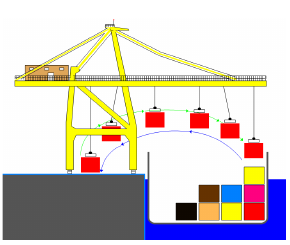
\includegraphics[width=2.5in]{esquema_grua.png}
  \caption{Esquemático de una grúa portuaria}
  \label{fig:grua}
\end{figure}

\begin{itemize}
 \item Traslación: Movimiento a lo largo del eje horizontal.
 \item Izaje: Movimiento a lo largo del eje vertical.
\end{itemize}
Mediante el control de ambos es posible llevar una
carga desde el muelle a su ubicación dentro del barco.


\subsection{Análisis del sistema físico}
\label{sec:fisica}
Para poder realizar el diseño de un controlador que
haga posible dicha tarea se cuenta con un modelo 
matemático del sistema. Tal  modelo se obtiene de la definición 
de un sistema de coordenadas y del análisis de los elementos 
actuantes.

Como se ve en la Fig.\ref{fig:ejes1} al designar un sistema de 
coordenadas se deben definir los valores máximos y mínimos 
para cada eje así como la ubicación del origen en el espacio.
Ademas existen otros elementos que dificultan el movimiento de
la carga como el caso de una viga testera a 15m. que define 
la altura mínima para la traslación en el muelle.

\begin{figure}[!t]
 \centering
  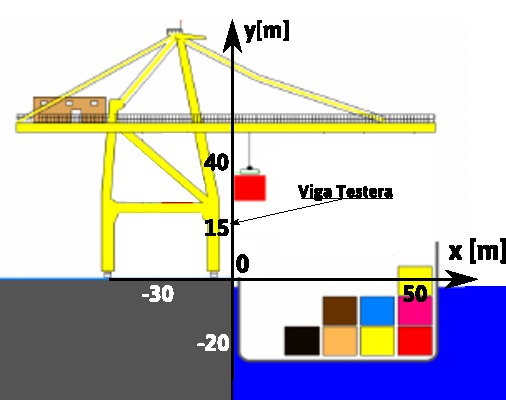
\includegraphics[width=2.5in]{EjesXY.pdf}
  \caption{Sistema de Coordenadas y valores característicos}
  \label{fig:ejes1}
\end{figure}

Se continua con el desarrollo del modelo analizando cada uno de
los elementos que actúan en el sistema:
\begin{itemize}
 \item Mecanismo de Traslación: dispositivo mecánico
 accionado por motores eléctricos que permite el 
 desplazamiento de la carga en el eje horizontal.
 \begin{itemize}
  \item Velocidad máx.: +/- 4.0 $m/s$ (cargado o sin carga).
  \item Aceleración máx: +/- 1.0 $m/s^2$ (cargado o sin carga).
  \item Carro (incluye sistema izaje):\\ 
  $m_c=50000 kg$;
  \item Radio primitivo de rueda: \\
  $R_w = 0.5 m$;
  \item Momento de inercia de ruedas (eje lento):\\ 
  $J_w = 2.0 kg.m^2$ 
  \item Caja reductora: relación \\
  $i=15:1$;
  \item Momento de inercia de motor y freno (eje rápido): 
  $J_m = 10 kg.m^2$;
  \item Fricción mecánica equivalente (eje rápido):\\
  $b_{eqm}=b_m+\dfrac{b_w}{i^2}=30 \dfrac{N.n}{rad.s}$.
 \end{itemize}

 \item Mecanismo de Izaje: Tambor giratorio sobre 
 el que se enrolla el cable de izaje.
 \begin{itemize}
  \item Velocidad máx.: +/- 1.5 $m/s$ (cargado) o +/- $3.0 m/s$ (sin carga).
  \item Aceleración max.: +/- 1.0 $m/s^2$ (cargado o sin carga).
  \item Radio primitivo de tambor: \\
  $R_d = 0.75 m$ (1 sola corrida de cable);
  \item Momento de inercia de tambor (eje lento):\\
  $J_d = 8.0 kg.m^2$.
  \item Caja reductora: relación \\
  $i=30.0:1$.
  \item Momento de inercia de motor y freno (eje rápido): $J_m = 30.0 kg.m^2$;
  \item Fricción mecánica equivalente (eje rápido):\\ 
  $b_{eqm}=b_m+\dfrac{b_d}{i^2}=18 \dfrac{N.n}{rad.s}$
 \end{itemize}

 \item Cable de Izaje: Cable de acero del cual cuelga
 la carga. Se encuentra todo el tiempo tensado.
 \begin{itemize}
  \item Cable elástico con rozamiento:\\
  $K_w=1,80.10^5~\dfrac{N}{m}\\$
  $b_w=3.10^3~\dfrac{N.s}{m}$
 \end{itemize}

 \item Carga suspendida: Es la inercia que se encuentra
 al final del cable de izaje. Se compone de la masa del
 elemento de agarre y de la carga nominal a transportar.
 \begin{itemize}
  \item Gancho vacío: $m_{l0}=15000 kg$ (sin carga)
  \item Gancho con Carga nominal: $m_l=65000 kg=(15000 + 50000 kg)$
 \end{itemize}

\end{itemize}

Debido a que nuestro modelo es plano, bidimensional
resulta interesante poder referir los movimientos 
giratorios de los motores eléctricos y del tambor
a coordenadas lineales.
 
\subsection{Modelo del sistema físico}
Para continuar en el desarrollo de un modelo matemático
necesitamos de un análisis de las fuerzas actuantes sobre
cada una de las partes antes descriptas. Mediante esta 
información presente en el diagrama de la Fig.\ref{fig:ejes}
se procede al desarrollo del modelo matemático de cada una 
de las partes:


\begin{figure}[!t]
 \centering
  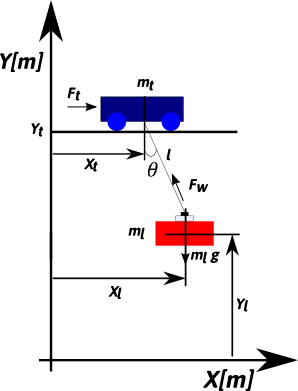
\includegraphics[width=2.5in]{trolley_carga.png}
  \caption{Análisis de fuerzas actuantes sobre el sistema}
  \label{fig:ejes}
\end{figure}


\subsubsection{Mecanismo de Traslación}
\label{sec:mecTras}
En el movimiento de traslación la masa en movimiento es la masa
total del sistema más las masas rodantes y sobre la que actúa 
la fuerza $F_t$, correspondiente a la tracción del trolley, y $F_w$, 
la fuerza de tensión del cable. Todos los rozamientos se reducen 
en $b_t$, coeficiente viscoso del mecanismo de traslación.
\begin{align}
    M_t \ddot{x_t}(t) &=  F_t(t) - b_t \dot{x_t}(t) + F_w(t) \sin \theta(t)\\
    \intertext{Donde:}
    M_t &= m_t + \dfrac{J_{w}+J_{m} i^2}{R_{w}^2} \\
    F_t &= \dfrac{T_{m} i}{R_{w}} \\
    b_t &= \dfrac{b_{eqm} i^2}{{R_{w}}^2}
\end{align}
Siendo $T_{m}$, el torque motor, nuestra variable manipulada en el sistema.

\subsubsection{Mecanismo de Izaje}
\label{sec:mecIza}
El mecanismo de izaje es rotatorio pero es mas conveniente expresarlo
en términos lineales. Donde $M_h$ es la inercia del mecanismo, 
$l_h$ representa el largo de cable
que se ha enrollado sobre el tambor, $F_h(t)$ la fuerza ejercida
sobre el cable por el accionamiento. Todos los rozamientos se reducen 
en $b_h$ coeficiente viscoso del mecanismo de izaje.
\begin{align}
    M_h \ddot{l_h}(t) &=  F_h(t) - b_h \dot{l_h}(t) - F_w(t) \\
    \intertext{Donde:}
    M_h &= \dfrac{J_{d}+J_{m} i^2}{R_{d}^2} \\
    F_h &= \dfrac{T_{m} i}{R_{d}} \\
    b_h &= \dfrac{b_{eqm} i^2}{{R_{d}}^2} 
\end{align}
Siendo $T_{m}$, el torque motor, nuestra variable manipulada en el sistema.
En la Fig.\ref{fig:fisica} se muestra el modelo en diagrama de bloques en Simulink.
\begin{figure}[!t]
 \centering
  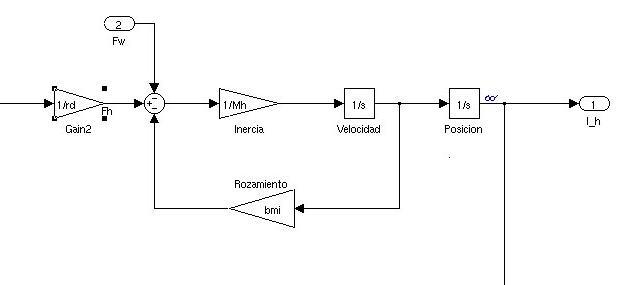
\includegraphics[width=2.5in]{analisis_sistema_fisico.jpeg}
  \caption{Diagrama de Bloques del Mecanismo de Izaje}
  \label{fig:fisica}
\end{figure}

\subsubsection{Cable de Izaje}
\label{subsec:cable}
Un cable de acero considerado equivalente elástico sin masa
propia es el elemento de unión entre el trolley y la carga
suspendida. Considerando la ley de Hooke y 
las perdidas por rozamientos viscosos la fuerza de tensión 
$F_w$ por es igual a:
\begin{align}
    F_w(t) &= K_w (l(t)-l_h(t)) + b_w(\dot{l}(t)-\dot{l_h}(t))
\end{align}
Donde $K_w$ es la constante elástica del cable y $b_w$ es la
constante que concentra los rozamientos internos del cable.

De manera geométrica se puede deducir el valor de $l$ y $\theta$ 
mediante el análisis de la Fig.\ref{fig:ejes}:
\begin{align}
    x_l(t) &=  x_t + l \sin \phi \\
    y_l(t) &=  y_t - l \cos \phi 
\end{align}
Despejando $l$ y $\theta$:
\begin{align}
    l &= \sqrt{(x_l - x_t)^2 + (y_t - y_l)^2} \\
    \tan \theta &= \dfrac{x_l - x_t}{y_t - y_l}
\end{align}

\subsubsection{Carga Suspendida}
Siendo $m_l$ la masa de la carga suspendida del cable
y sobre la que solo actúan la fuerza $F_w$ y
su peso, el modelo matemático es el siguiente:
\begin{align}
    m_l \ddot{x_l}(t) &=  -F_w(t) \sin \theta(t) \\
    m_l \ddot{y_l}(t) &=  F_w(t) \cos \theta(t) - m_l g 
\end{align}

\subsection{Condiciones iniciales y  paŕametros del sistema}
\label{sec:condiniciales}

Para poder comenzar a realizar los controladores se debe conocer cuales serán 
las condiciones iniciales de nuestro modelo.

\begin{itemize}
 \item Profundidad del barco: $prof \_ barco$
 
 Se pensó en esta variable teniendo en cuenta de que los barcos que debemos cargar pueden
 presentar dimensiones diferentes.
 \item Altura del container: $hContainer$
 
 Esta variable sirve para saber hasta donde hay que descender la carga, dependiendo del 
 número de contariners dejados.
 \item Ancho del container: $wContainer$
 
 Esta variable sirve para apartir del ancho del container saber hasta donde 
 hay que trasladar la carga, dependiendo del número de columna a la que hay 
 que ir.
 
 \item Posición inicial de la carga: $yl0 =  hContainer + 1$
 
 La posición inicial de la carga se decidió que fuera de la altura del 
 container más un metro de seguridad y para que el cable este cargado.
 \item Altura máxima de la carga: $yl\_max$
 
 Es la altura máxima a la que la carga puede subir. 
 \item Altura mínima de la carga: $yl\_min = prof\_barco - 1.3$
 
 Es la posición mínima que puede tener la carga, esta posición es dentro de la cubierta
 del barco
 \item Altura de la columna: $yt0 = 45 $
 
 La viga sobre la que se desplaza el trolley esta ubicada 45 metros 
 sobre el nivel del puerto. Es a partir de esta coordenada que el cable se desenrolla.
 \item Número de columnas: $numColumna$
 
 Esta variable tiene como objetivo poder variar el número de columnas de contenedores
 posibles en el barco. El objetivo es poder aceptar diferentes barcos.
 \item Número de containers por columna: $NumContainter = [0 \, 0 \, 0 \, 0 \, 0]$
 
 El objetivo de este vector es guardar el número de containter existente en cada columna.
 Esto nos permite saber hasta donde descender debido a que conocemos el alto de los 
 contenedores evitando de esta manera colisiones.
 \item Posición inicial del carro: $xt\_h$
 
 El carro comienza quince metros dentro del puerto.
 \item Longitud inicial de cable desenrollado:
 
 $lh\_h = yt0-yl0- \dfrac{mL \, g}{Kw} $ 
 
 Para asegurar una posición inicial de la carga el cable debe estar desenrollado una 
 constante que tiene en cuenta cuanto el cable se necesita estirar para ejercer una fuerza
 tal que contrarreste el peso de la carga. Esta expresión fue obtenida a partir de las 
 expresiones presentadas en la sección \ref{subsec:cable}. Esto nos asegura que el cable 
 en el instante inicial ya esta precargado y no hay movimiento del cable en la dirección
 $y$.
 
 \item Longitud mínima de cable desenrollado: 
 
 $lh\_min = yt0 - yl\_max-\dfrac{mL \, g}{Kw}$
 
 Para asegurar que la carga no va a superar su posición máxima definida en la variable
 $yl_max$, debemos tener en cuenta al momento de enrollar el cable cuanto necesito que este
 se estire para contrarrestar el peso de la carga.
 
 \item Posición objetivo del carro:
 
 $xt\_g= (numColumna + 0.5) \, wContainer$
 
 La posición final del carro depende del numero de columna  a la que deba ir la carga.
 \item Longitud objetivo del cable desenrollado:

 $lh\_g = yt0 + yl\_min $
 $-  (hContainer \, numContainer \, (numColumna))$
 $- \dfrac{mL \, g}{Kw}$
 
 Para dejar la carga cerca del lugar deseado en donde el operador toma el mando de la
 grúa para proceder con la descarga debemos tener en cuenta el número de containers que
 se encuentran depositados y cuanto se va a estirar el cable.
 
 \item Fuerza de precarga: $Fh0$
 
 Como se explicará en la sección \ref{sec:rescontrolador} en el controlador se utilizó una
 fuerza de precarga para no sufrir un descenso de la carga cuando se comienza un recorrido
 y es el control automático el que toma el mando.
 
\end{itemize}

\subsection{Limitador de velocidad y aceleración}
\label{sec:limites}
Una de las imposiciones del trabajo es un límite en la velocidad y la aceleración como se
mencionó en el capítulo \ref{sec:fisica}.

Para poder asegurar no superar los límites de velocidad la consigna de posición no puede 
ser un salto en escalón y su razón de cambio no puede superar los valores dados como 
objetivo. 
Por otro lado para cumplir con los límites de velocidad impuestos la consigna de velocidad 
no puede ser un salto en escalón y su razón de cambio debe estar limitada.

En la fig. \ref{fig:bloque_consigna_pos} se puede observar el bloque en Matlab-Simulink
que nos entrega una consigna de posición con las características necesarias para no
superar los límites de velocidad y aceleración.

\begin{figure}[!t]
 \centering
  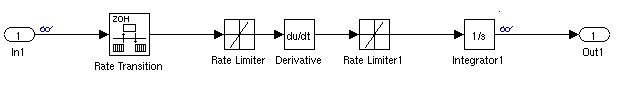
\includegraphics[width=2.5in]{bloque_consigna_posicion.jpeg}
  \caption{Bloque Matlab-Simulink para la consigna de posición.}
  \label{fig:bloque_consigna_pos} 
\end{figure}

La consigna de posición entregada al controlador, resultado del bloaque de Matlab 
se observa en la fig. \ref{fig:consigna_pos}. En esta se observan como al iniciar y
al finalizar el desplazamiento se describen dos parábolas debido al limite de 
aceleración y se forma una rampa en el centro por la limitación de la velocidad.
\begin{figure}[!t]
 \centering
  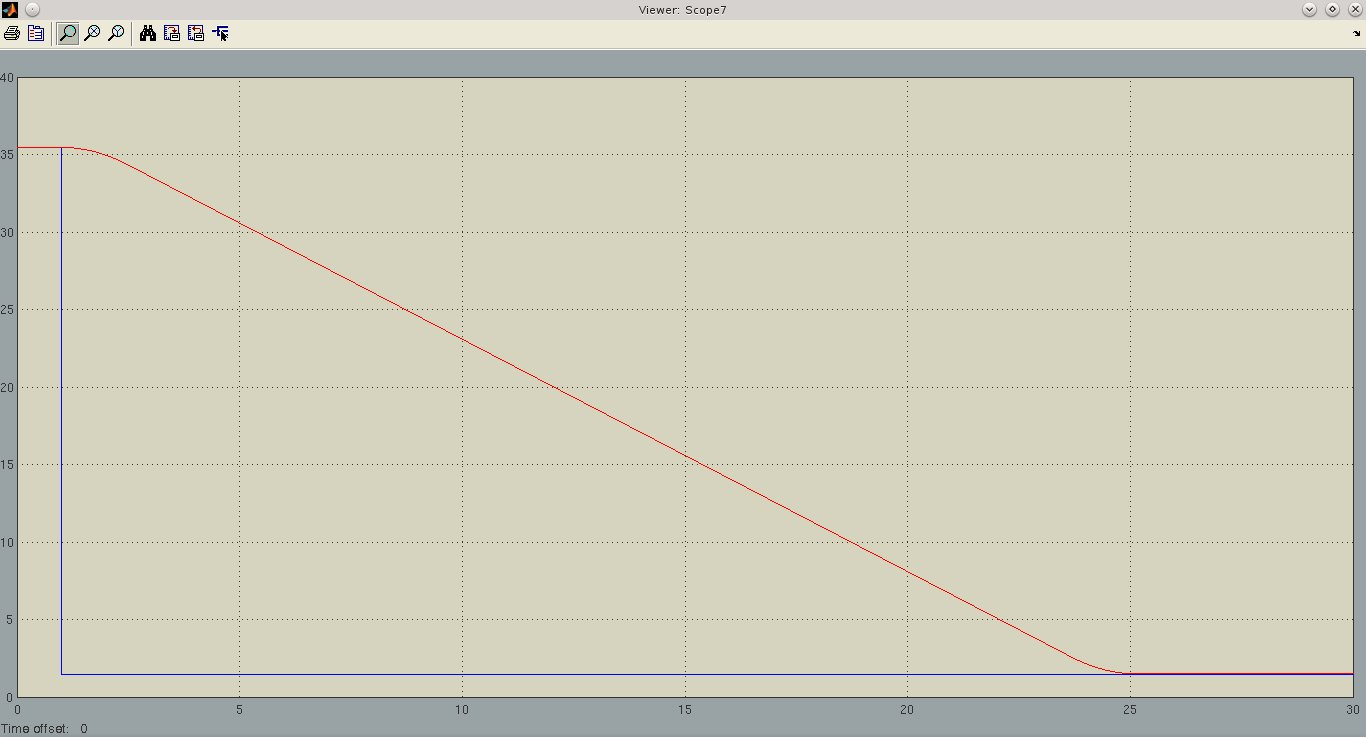
\includegraphics[width=2.5in]{consigna_posicion.jpeg}
  \caption{Gráfico de la consigna de posicíon en funcion del tiempo}
  \label{fig:consigna_pos}
\end{figure}

Por último en la fig.\ref{fig:atenuaciona} se observa la aceleración al describir 
la trayectoria anterior, cumpliendo con las condiciones demandadas y en la fig. \ref{fig:atenuacionv} se 
muestran los resultados para la velocidad. Esta pertenece al sistema de izaje.

\begin{figure}[!t]
 \centering
  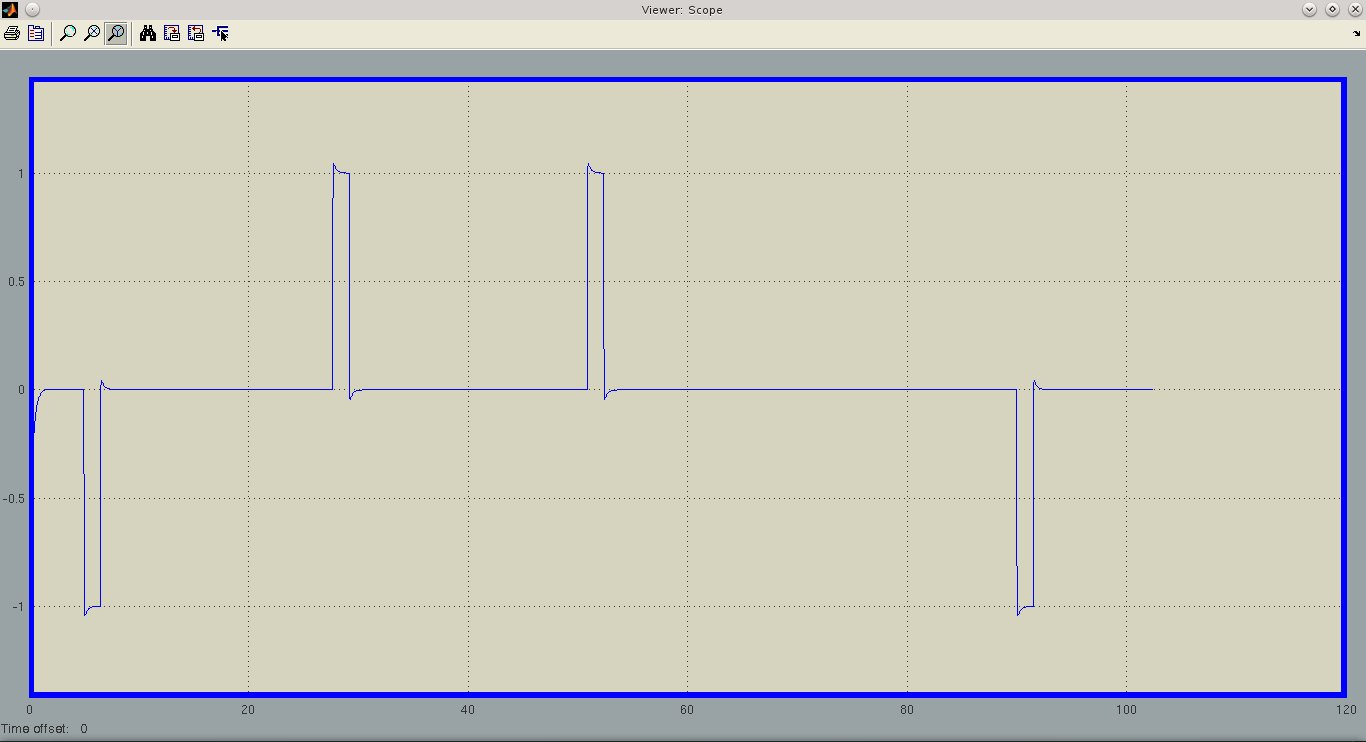
\includegraphics[width=2.5in]{atenuaciona.jpeg}
  \caption{Gráfico de la limitación de la aceleración}
  \label{fig:atenuaciona}
\end{figure}

\begin{figure}[!t]
 \centering
  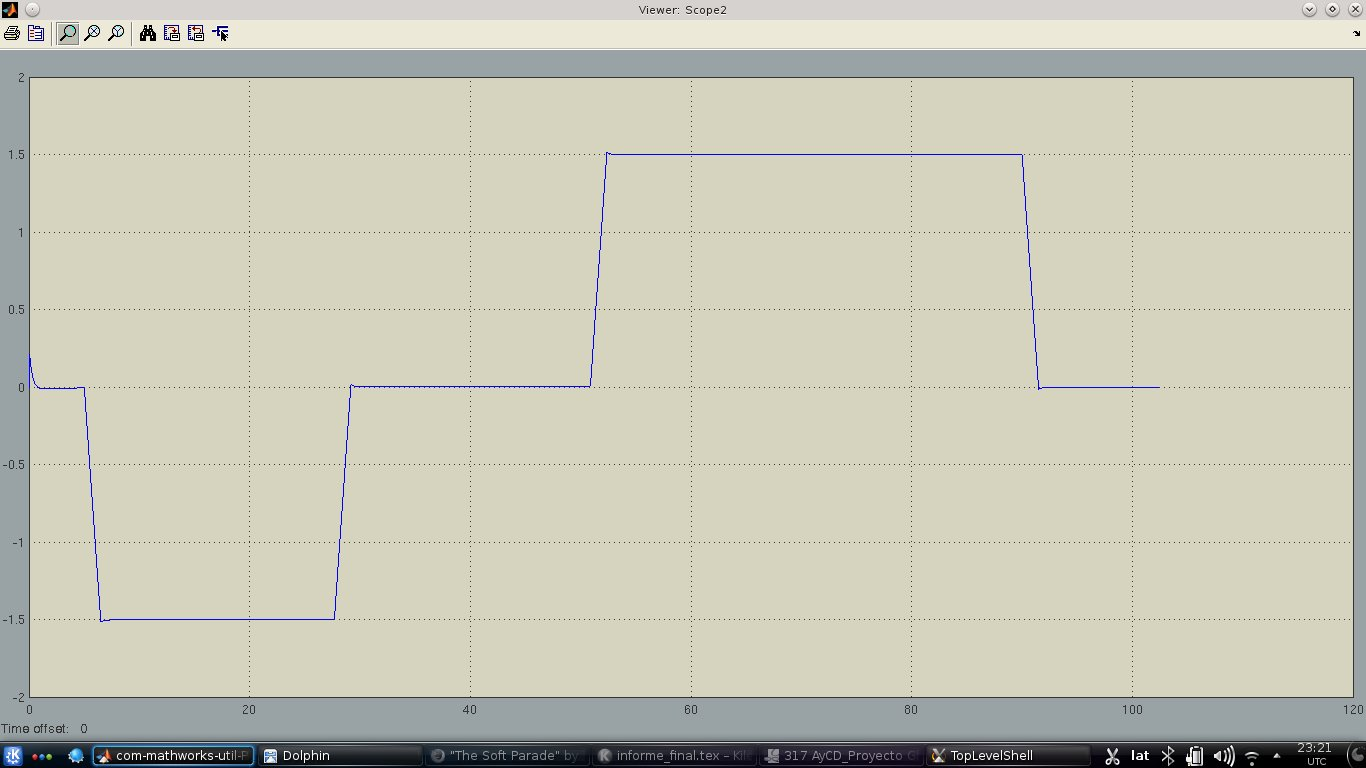
\includegraphics[width=2.5in]{atenuacionv.jpeg}
  \caption{Gráfico de la limitación de la velocidad}
  \label{fig:atenuacionv}
\end{figure}

\subsection{Controladores de tipo PID}
Luego de analizar el modelo físico se procedió a realizar un controlador por cada motor.
Debemos ser capaces de conducir la carga hasta una posición, si bien la acción de 
tomar la carga y dejar la misma es realizada de manera manual, es necesario que de manera
automática la carga llegue a la posición deseada. 

Como se explicará en las próximas secciones el controlador supervisor global enviará
una consigna de posición a la cual debe llegar nuestro actuador.

En una primera versión del trabajo este controlador supervisor enviaba una consigna de 
velocidad, la cual era seguida de acuerdo a un bucle de control PID. Entre las ventajas
que encontramos en esta solución se encontraba una parada de emergencia sencilla, debido
a que era suficiente con enviar una consigna de velocidad cero. Sin embargo luego
de analizar aquellos resultados se decidió enviar desde el supervisor consignas de 
posición, las cuales son alcanzadas a través de un controlador de tipo PID. 
Se decidió este tipo de controlador luego de analizar otros métodos.

La acción de control PID es el resultado de la suma de una ganancia proporcional multiplicada
por el error, una ganancia integral multiplicada por la integral del error y una ganancia
derivativa multiplicada por la derivada del mismo.

Se demostrará de manera general el camino seguido para obtener el valor de las ganancias para 
los controladores dado que la metodología es la misma en ambos casos. Para poder obtener este
controlador se opero de la siguiente manera:

\subsubsection{Análisis del sistema}
A partir del modelo físico de un motor eléctrico de corriente continua:
\begin{align}
  J_m \, \dot{\omega (t)} &= T_m - T_l - b \,{\omega}(t)\\
  \dot{\theta} &={\omega} (t)
\end{align}
Donde $J_m$ es la inercia del motor, $T_m$ es el torque del motor y $b$ es
el coeficiente de rozamiento dinámico. $\theta$ es el ángulo girado por el 
eje del motor.

Que en el dominio $s$ :
\begin{align}
  J_m \, s \, \omega (s) &= T_m (s) \,- \, T_l(s) \, -\,b\,\omega(s)\\
  s \, \theta (s) &= \omega (s)
\end{align}

Se desean obtener los valores correctos de las ganancias
del controlador, tal que la salida del sistema siga a la 
consigna del controlador.

\subsubsection{Función de transferencia del sistema}
Para ello analizamos cuales son las entradas y salidas del sistema.\\
Entrada: $\theta^*$ \\
Salida: $\theta \rightarrow$  variable controlada\\

El error esta definido como la diferencia entre la entrada y la salida del sistema:
 \begin{align}
  e_\theta (t) &= \theta^* (t) \,-\, \theta (t)
%  \frac{\mathrm d}{\mathrm d t} \left( e_\theta \right) &= \omega^* (t) - \omega(t)
 \end{align}
 
Dado que el modulador de torque del motor eléctrico es modelado como una ganancia 
unitaria $G_T(s)$ por las condiciones del mismo (ancho de banda muy grande en 
comparación con el sistema controlado), el torque motor $T_m$ es igual a
 \begin{align}
%   (J_m \,s^2 \, + \,b\, s) \theta (s) &= T_m (s) - T_l (s)\\
   T_m (s) &= G_T (s) \big[ k_p + k_i \, \dfrac{1}{s} + \,k_d \,s] \, e_\theta (s) \\
           &= G_T (s) \big[ k_p + k_i \, \dfrac{1}{s} + \,k_d \,s] \, [\theta^* (s) \,-\, \theta (s)]
 \end{align}

Igualando y operando matemáticamente $T_m$, se obtienen las siguientes funciones
de transferencia:

 \begin{align}
    \dfrac{\theta(s)}{\theta^*(s)} = \dfrac{G_T(s)\big[k_d s^2 + k_p s + k_i]}{J_m s^3 + [b_m + G_T(s) k_d] s^2 + G_T (s)[k_p s + k_i]}\\
    \dfrac{\theta}{T_l} = - \dfrac{s}{J_m s^3 + [b_m + G_T(s) k_d] s^2 + G_T(s)[k_p s + k_i]}
 \end{align}
 
 
\subsubsection{Polos de la función}
En este punto somos capaces de elegir los polos de ambas funciones de transferencia de la 
siguiente manera:
\begin{itemize}
 \item $P_1 < 0$ 
 \item $P_2$ y $P_3$ complejos conjugados.
\end{itemize}
Dicha ecuación en forma factorizada se escribe como:
\begin{align}
    &=(s - P_1)(s - P_2)(s - P_3)\\
    &=(s - P_1)(s^2 + 2 \xi {\omega}_n s + {{\omega}_n}^2)\\
    \intertext{Desarrollando, obtenemos la expresión} 
    &=s^3 + (2 \xi {\omega}_n - P_1) s^2 + ({{\omega}_n}^2 - 2 \xi {\omega}_n P_1) s - {{\omega}_n}^2 P_1
\end{align}



\subsubsection{Ganancias Kp, Ki y Kd}
Para obtener las ganancias Kp, Ki y Kd se igualan termino a termino:
\begin{align}
  &=J_m s^3 + (b_m + G_T(s) k_d) s^2 + G_T (s)(k_p s + k_i)\\
  &= s^3 + (2 \xi {\omega}_n - P_1) s^2 + ({{\omega}_n}^2 - 2 \xi {\omega}_n P_1) s - {{\omega}_n}^2 P_1
\end{align}

Ganancia proporcional: 
\begin{align}
  k_p = ({{\omega}_n}^2 - 2 \xi {\omega}_n P_1) J_m
\end{align}

Ganancia integral:
\begin{align}
  k_i = (P_1 {{\omega}_n}^2) J_m
\end{align}

Ganancia derivativa:
\begin{align}
  k_d = (2 \xi {\omega}_n - P_1) J_m - b_m
\end{align}
Aplicando estas expresiones a los modelos físicos de la sección \ref{sec:mecTras} y 
\ref{sec:mecIza} tenemos:\\
Mecanismo de traslación
\begin{align}
  k_p &= ({{\omega}_n}^2 - 2 \xi {\omega}_n P_1) M_t\\
  k_i &= (P_1 {{\omega}_n}^2) M_t\\
  k_d &= (2 \xi {\omega}_n - P_1) M_t - b_t
\end{align}
Mecanismo de izaje
\begin{align}
  k_p &= ({{\omega}_n}^2 - 2 \xi {\omega}_n P_1) M_h\\
  k_i &= (P_1 {{\omega}_n}^2) M_h\\
  k_d &= (2 \xi {\omega}_n - P_1) M_h - b_h
\end{align}



\subsection{Parada de emergencia}
Sistemas de gran envergadura presentan frenos mecánicos para no estar forzando el motor
y tener una mayor seguridad. Se pensó en este trabajo que en una situación de riesgo
es necesario detener el sistema de forma segura antes de aplicar los frenos mecánicos.

Dado que el controlador que acabamos de describir solo controla posición, 
no nos daba la seguridad de detener los motores de manera sencilla y rápida. 
Decidimos realizar un controlador de tipo PID 
pero de velocidad. Este sistema actúa solamente en caso de emergencia. A continuación se 
detalla el esquema de Matlab-Simulink (Ver Fig.\ref{fig:ControlVel}).

%%%%%%%%%%%%%%%%%%%%%%%%%%%%%%%%%%%%%%%
%imagen del control de velocidad
%%%%%%%%%%%%%%%%%%%%%%%%%%%%%%%%%%%%%%%%
\begin{figure}[!t]
 \centering
  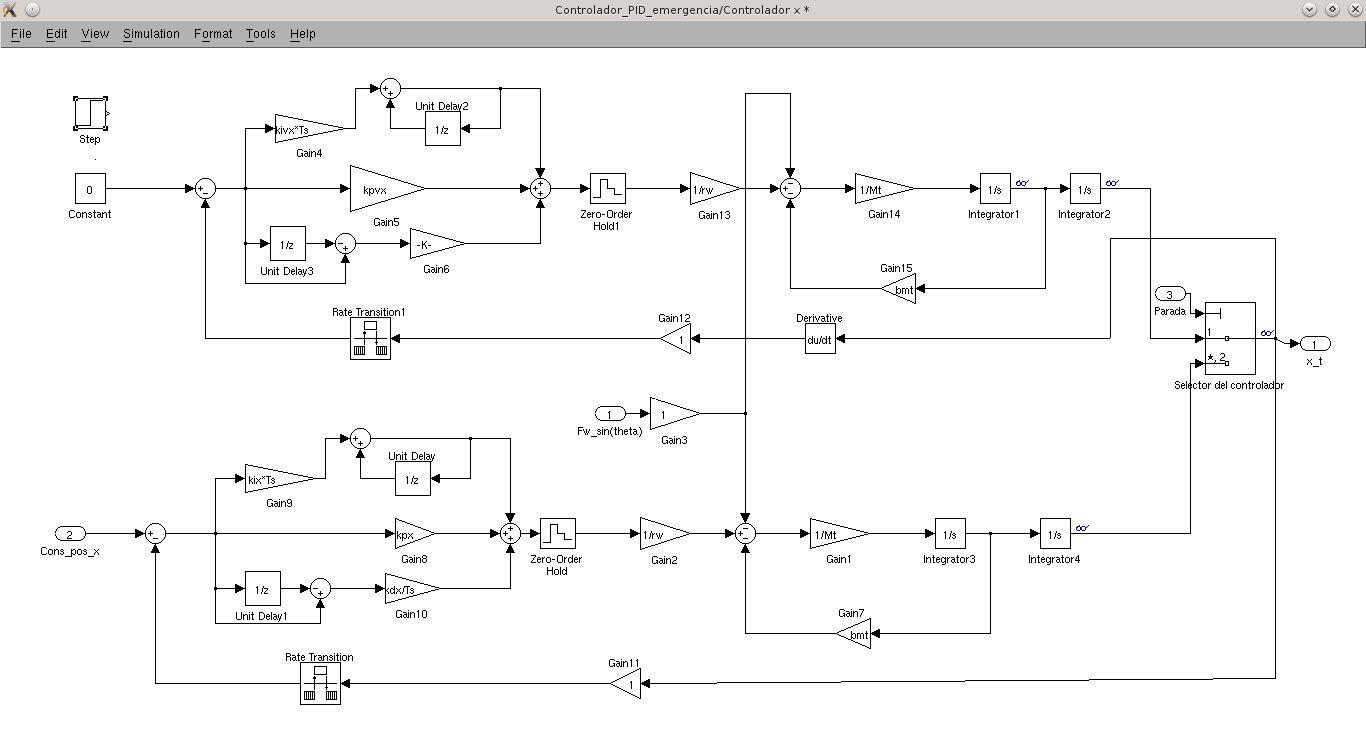
\includegraphics[width=2.5in]{Test_Controlador_emergencia1.jpeg}
  \caption{Diagrama del controlador de posición y de velocidad(Emergencia)}
  \label{fig:ControlVel}
\end{figure}

Para poder obtener las ganancias se siguió el método de Ziegler-Nichols en el que se 
realiza un análisis de la respuesta del sistema a una perturbación en escalón.

Como se explicara en la sección \ref{sec:MaqEstados}, mediante la bandera "Emergencia" 
se tienen la capacidad de decir que controlador tiene el mando del sistema y su 
correspondiente consigna.

Analizando los resultados anteriores se busco otra solución en la cual se retroalimenta 
el estado actual del sistema como consigna del controlador. De esta manera el error es 
cero. Se debe tener en cuenta la perturbación $F_w$ y es por ello que la consigna que 
llegue al modulador de torque $G_t$ debe ser igual igual a esta. Ver Fig.
\ref{fig:testVel} 

\begin{figure}[!t]
 \centering
  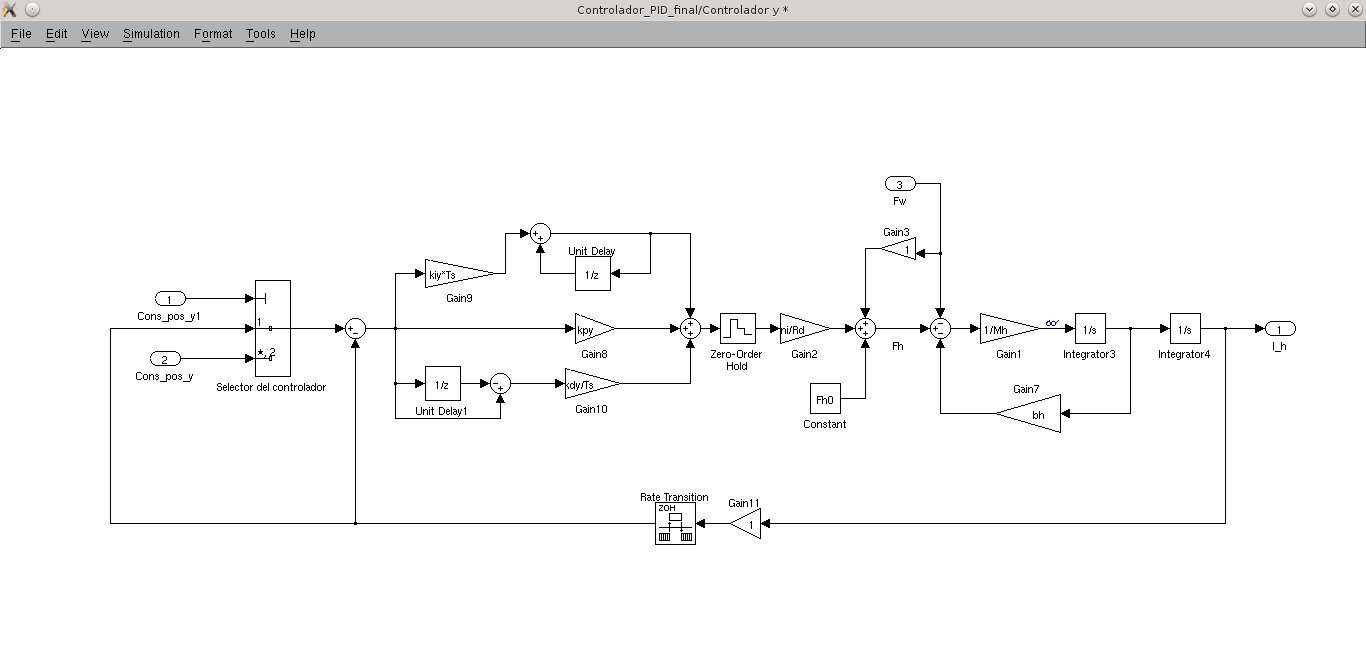
\includegraphics[width=2.5in]{Controlador_precarga_velocidad.jpeg}
  \caption{Modelo Simulink del controlador de izaje en el eje Y con precarga y sistema de 
  emergencia}
  \label{fig:testVel}
\end{figure}

Observando las soluciones propuestas y los resultados obtenidos se descubrió que esta 
retroalimentación podía hacerse directamente en la máquina de estados. Para ello se debe
enviar como consigna de posición la posición actual al momento de entrar al estado 
emergencia.
Esto se explicará en el capítulo \ref{sec:MaqEstados}. En la fig. \ref{fig:paradaemergencia} se muestra
la consigna $cons\_xt=xt$ donde $xt$ es la retroalimentación de la posición y $cons\_lh=lh$
donde $lh$ es la retroalimentación de los metros desenrollados de cable.

\begin{figure}[!t]
 \centering
  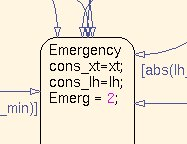
\includegraphics[width=1in]{parad_de_emergencia_state.jpeg}
  \caption{Imagen del estado emergencia en la máquina de estados}
  \label{fig:paradaemergencia}
\end{figure}


\subsection{Análisis en tiempo discreto}
Hasta este momento hemos presentado nuestro trabajo en el controlador en tiempo continuo.
El objetivo de este trabajo es presentar una solución digital y es por ello que se adaptó
el modelo de Matlab de tiempo discreto a digital, cumpliendo con las necesidades del
trabajo. 

La adaptación que se realizo fue la siguiente:
\begin{itemize}
 \item Debemos discretizar los valores de la entrada. En esta nueva situación del sistema 
vamos a dividir el tiempo continuo en pequeños intervalos, esto nos inhibe de conocer
el estado del sistema en cada momento. Al diseñar un controlador digital asumimos este
riesgo y se deben tomar los recados necesarios para cumplir con nuestros objetivos de 
seguridad brindando un sistema fiable. Esto se resume a realizar un sistema de control 
lo suficientemente rápido en función de la variación de las variables del proceso.

El teorema de muestreo nos dice que el tiempo de muestreo debe ser:

$ f_s > 2*BWcontrolador $

En la práctica esta relación es aún mayor.

\item A su vez la salida de un sistema digital es discreta. Esto implica 
que nuestro sistema de control presenta una salida escalonada. Por ende, 
actuando, sobre el sistema de manera diferente a un sistema continuo. Otra 
vez es importante tener en cuenta el tiempo con el cual el controlador actualiza
la señal de salida.
\end{itemize}

Se presenta a continuación el camino para transformar un PID continuo a uno discreto:
\begin{itemize}

 \item Acción integral
  \begin{align}
    u_i (t) =& {k_i \int\limits_0^t e(t) dt} + u_{i0}
    \intertext{Para un instante de muestreo:} \
    u_i (t_k) =& k_i \big[{\int\limits_{0}^{t_k} e(t) dt} + I_0] \\
              =& k_i \big[\int\limits_{t_{k-1}}^{t_k} e(t) dt + \int\limits_0^{t_{k-1}} e(t) dt + I_0]\\
    u_i(t_{k-1}) =&  k_i \int\limits_0^{t_{k-1}} e(t) dt + I_0 \\
    u_i (t_k) =& k_i \int\limits_{t_{k-1}}^{t_k} e(t) dt + u_i (t_{k-1})\\
              =& k_i~e(t)~T_s + u_i (t_{k-1})
    \end{align}
 \item Acción derivativa
  \begin{align}
    u_d (t_k) =& k_d \dfrac{d\,e(t_k)}{dt}\\
              =& k_d \dfrac{e(t_k)-e(t_{k-1})}{Ts}
  \end{align}
\end{itemize}
Donde $T_s$ es el tiempo de muestreo igual a $T_s=\dfrac{10}{\omega_n}$
En la Fig.\ref{fig:controlador} se observa el diagrama de bloques de un 
controlador discreto.

\begin{figure}[!t]
 \centering
  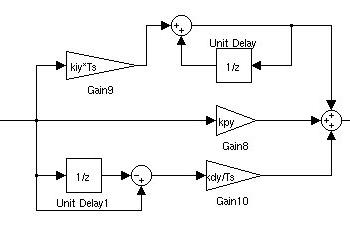
\includegraphics{controlador_posicion.jpeg}
  \caption{Diagrama de bloques de un controlador discreto}
  \label{fig:controlador}
\end{figure}


\subsection{Adaptación del programa en Matlab-Simulink}
Se deben agregar dos bloques de función en el programa de Matlab para transformar nuestro 
controlador en tiempo continuo al discreto.
\begin{itemize}
\item Al ingreso del controlador: Rate Transition(Ver Fig.\ref{fig:rate})
\begin{figure}[!t]
 \centering
  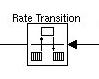
\includegraphics{rate.jpeg}
  \caption{Bloque Rate Transition}
  \label{fig:rate}
\end{figure}

De acuerdo a la descripción de Matlab el bloque se encarga de transferir datos 
entre sistemas que trabajan a una frecuencia diferente. El trabajo del bloque es mantener a 
la salida un valor que se encontraba a la entrada en el momento del muestreo.


\item A la salida del controlador: Zero-order hold (Ver Fig.\ref{fig:zero})
\begin{figure}[!t]
 \centering
  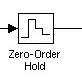
\includegraphics{zero_order.jpeg}
  \caption{Bloque Zero Order Hold }
  \label{fig:zero}
\end{figure}
Según Matlab el bloque retiene su entrada durante un período de tiempo especificado.
\end{itemize}

Con estos dos elementos ademas de la transformación de las acciones proporcionales, 
integrales y derivativas se realizó el controlador en tiempo discreto.

\subsection{Máquina de estados finitos}
\label{sec:MaqEstados}
Una máquina de estados puede describirse como el modelo de comportamiento de un sistema
en que los sucesivos estados dependen al mismo tiempo de las entradas del sistema y 
del estado en el que se encuentra. 

Para poder realizar la máquina se realizaron tres versiones hasta poder obtener el
resultado final. A continuación se presenta una breve descripción de las mismas.

\begin{itemize}
 \item En la primera versión se busco que la máquina fuera capaz de ubicar la carga en 
 el barco. Lo que debía realizar luego de salir del estado manual (en el que el operario
 toma la carga) es ir a una posición conocida y segura, para a partir de ese momento 
 comenzar a avanzar, desde este punto hasta el punto más alto permitido. A partir de 
 este momento se comienza a trasladar el carro en el eje $x$, hasta su posición final en el 
 eje x, y por ultimo comienza su descenso hasta la posición final en el eje y. El ultimo estado
 era nuevamente manual, donde el operario debería dejar la carga.
 
 \item La segunda versión de la máquina de estados tomaba lo realizado en la primera versión 
 pero además agregaba un grupo de estados que representaban el camino de regreso, ascenso el el
 eje y, traslación en el eje $x$ y descenso hasta el muelle. El problema general se concibe de
 manera que la grúa siempre va a realizar un ciclo completo, ida hacia el barco y regreso al muelle. 
 
 \item La tercer y ultima versión hasta el momento se le agregan las señales de emergencia en las 
 que detienen el sistema y le avisan al operario que el sistema no esta respondiendo de una manera
 esperada.
 
\end{itemize}


La máquina de estados realizada se describe en su forma de
diagrama de estados finitos en la Fig.\ref{fig:dig_control}. A continuación y haciendo 
referencia a los nombres de este diagrama se detalla el comportamiento en modo automático 
de nuestra grúa tipo pórtico:

Tomando como inicio el momento en el cual el operario, después de haber intervenido en 
el proceso de enganche y primera elevación de la carga, pone el sistema en modo 
automático, este responde de la siguiente manera:
\begin{itemize}
 \item $Automatic~Control$: Entrada en el Modo Automático. Nuestro sistema viene de
 haber estado controlado por el operario y por ello es necesario que el sistema se 
 reoriente para cumplir con su tarea. Para esto evalúa si su posición actual es 
 próxima a alguna de sus dos posiciones conocidas:
 \begin{itemize}
  \item $Home$: Un punto ubicado sobre el muelle a una altura por encima del 
  area de trabajo usual del operario.
  \item $Goal$: El punto de destino sobre el barco para depositar la carga que se esta
  transportando.
 \end{itemize}
 Si ninguna de las dos posiciones se encontraran cerca esto es considerado como un error 
 del operario que ha accionado el modo automático y el autómata entra el modo
 de $Emergency$.
 \item $Approach~Home$ y $Approach~Goal$: Estando cerca de los puntos conocidos  
 ($Near~Home$ y $Near~Goal$) nos acercamos a estos.
 \item $Home~Climb$ y $End~Climb$: A continuación, tras encontrarnos en un punto conocido 
 y seguro $At~Home$ y $At~Goal$ procedemos a desplazarnos
 en el eje $Y$ hasta la posición mas alta $Highest$.
 \item $Go$ y $Return$: Al alcanzar la coordenada de mayor altura de nuestra 
  estructura $Highest$ es seguro proceder a desplazarnos en el eje $X$ hasta la posición 
  del destino sobre este eje: $ X~Goal$ y $X~Home$ respectivamente.
 \item $Descend~Goal$ y $Descend~Home$: al encontrarnos por encima de nuestro destino 
 podemos descender de manera segura hasta alcanzar la posición $At~Goal$ y $At~Home$
 en cada caso.
 \item $Wait$: Luego de haber llegado al destino esperamos la señal del 
 operador $Manual$ para dar paso al control manual del sistema.
  \item $Emergency$: Como se describió una situación anormal del sistema lleva al mismo
  a un estado de emergencia el cual detiene los motores. Pero no solo una situación del
  sistema lleva a este estado, también el operario puede llevar al sistema al estado
  emergencia mediante la activación de un switch. Para salir de este estado el operario
  debe dar la señal de que se tiene conocimiento de que el sistema entro a un estado de 
  emergencia y pasará de esta forma a un estado manual, siguiendo así con su funcionamiento
  normal.
\end{itemize}

\begin{figure*}[!t]
  \centering 
  %\resizebox{2.5in}{!}{    
      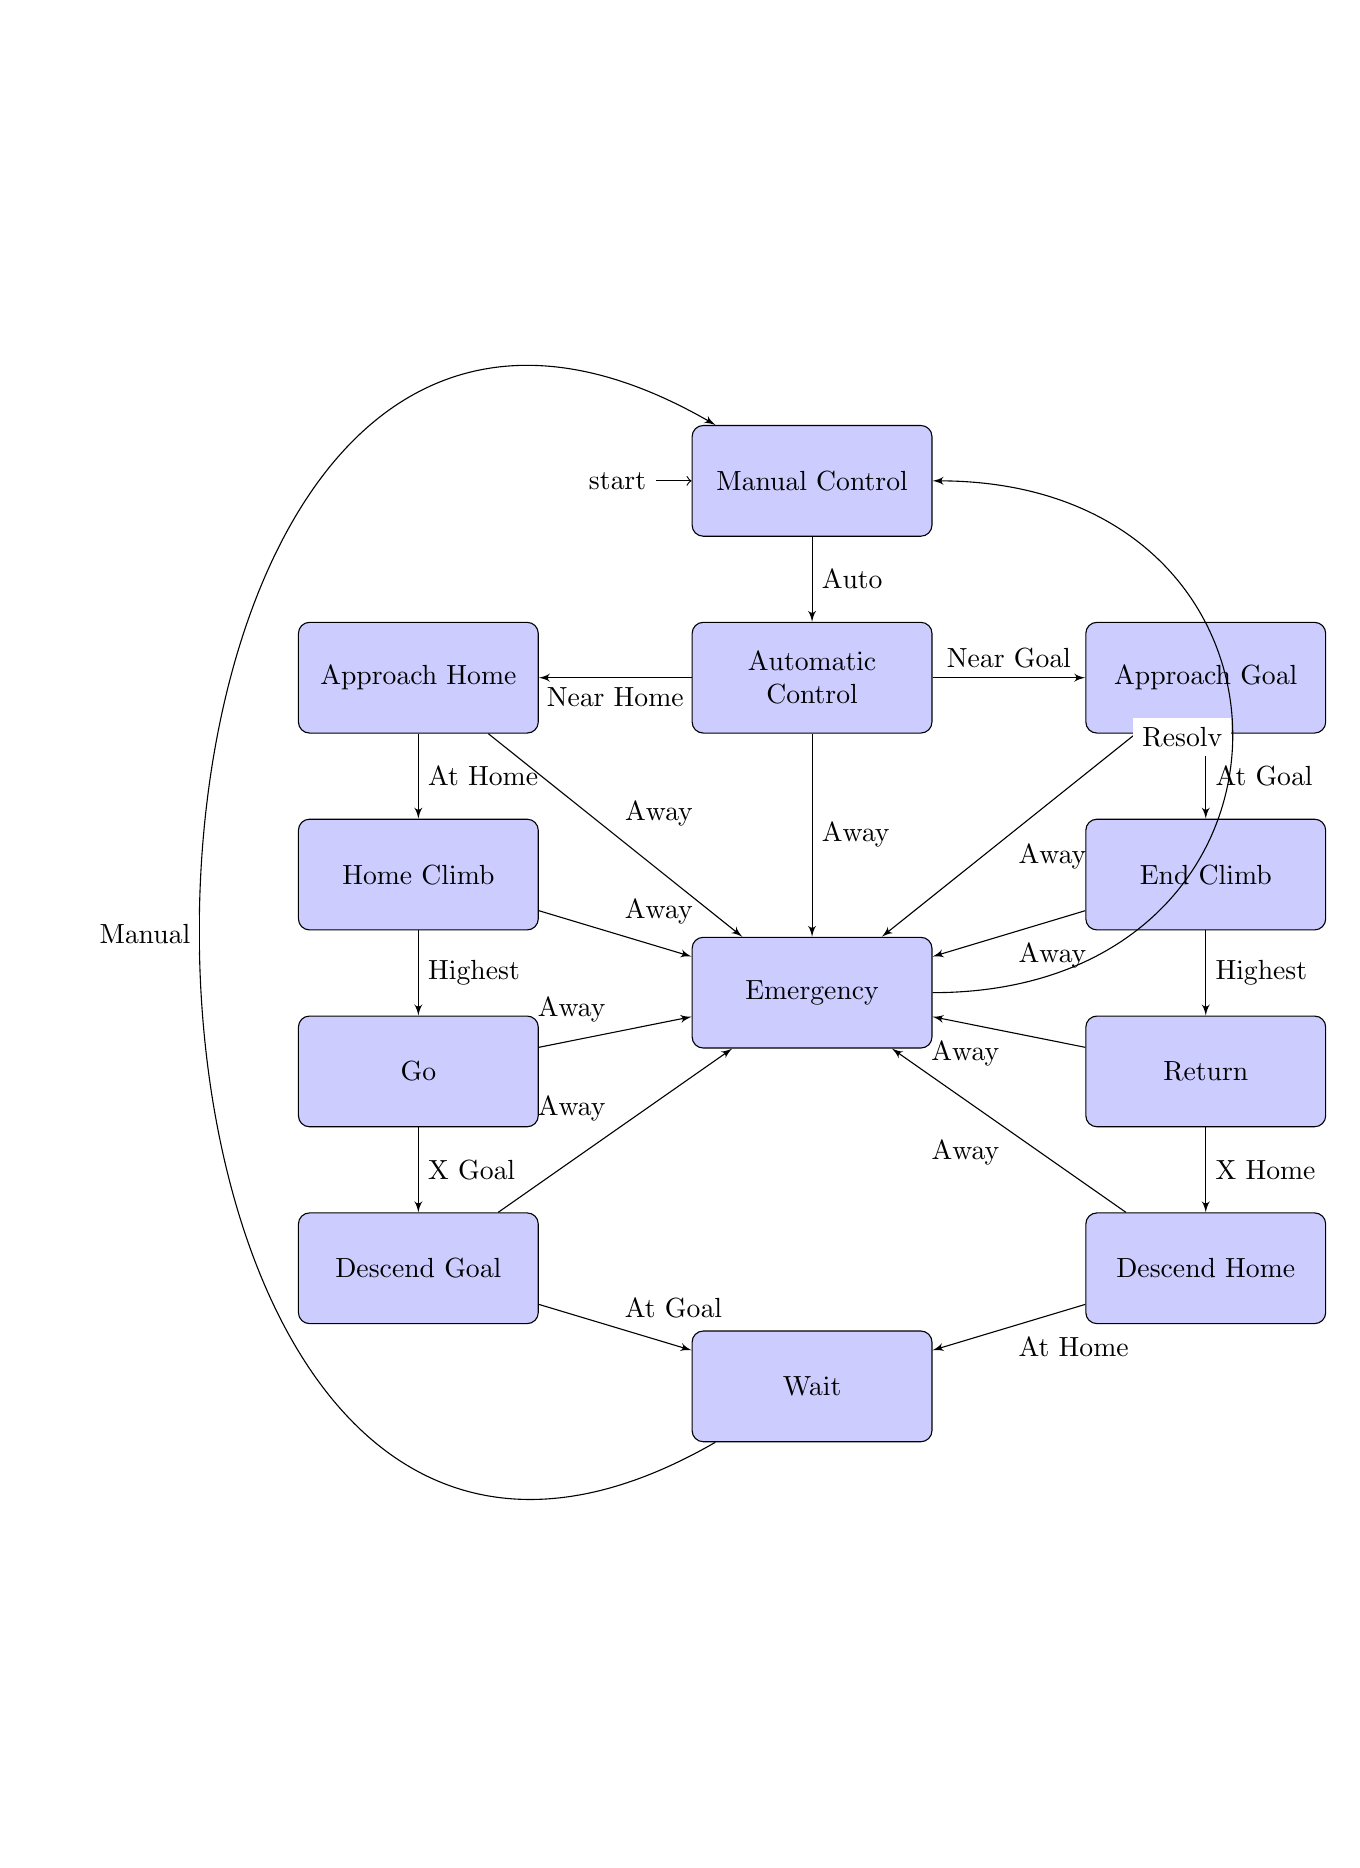
\begin{tikzpicture}[node distance = 2.5 cm, auto]
	  % Nodes
	  \node [initial,block] (init) {Manual Control};
	  \node [block, below of=init] (auto) {Automatic Control};
	  \node [block, below of=auto, node distance = 4cm] (emergency) {Emergency};
	  \node [block, left of=auto,node distance = 5 cm] (apHome) {Approach Home};
	  \node [block, below of = apHome] (upHome) {Home Climb};
	  \node [block, below of= upHome] (go) {Go};
	  \node [block, below of= go] (descendEnd) {Descend Goal};
	  \node [block, right of= auto, node distance = 5 cm] (apEnd) {Approach Goal};
	  \node [block, below of= apEnd] (upEnd) {End Climb};
	  \node [block, below of= upEnd] (return) {Return};
	  \node [block, below of= return] (descendHome) {Descend Home};
	  \node [block, below of= emergency, node distance = 5 cm] (end) {Wait};
	  %Uso Normal
	  \path [line] (init) -- node {Auto} (auto);
	  \path [line] (auto) -- node {Near Home} (apHome); 
	  \path [line] (apHome) -- node {At Home} (upHome);
	  \path [line] (upHome) -- node {Highest} (go);
	  \path [line] (go) -- node {X Goal} (descendEnd);
	  \path [line] (descendEnd) -- node {At Goal} (end);
	  \path [line] (auto) -- node {Near Goal} (apEnd);
	  \path [line] (apEnd) -- node {At Goal} (upEnd);
	  \path [line] (upEnd) -- node {Highest} (return);
	  \path [line] (return) -- node {X Home} (descendHome);
	  \path [line] (descendHome) -- node {At Home} (end);
	  %Emergencia
	  \path [line] (auto) -- node {Away} (emergency);
	  \path [line] (apHome) -- node {Away} (emergency);
	  \path [line] (upHome) -- node {Away} (emergency);
	  \path [line] (go) -- node {Away} (emergency);
	  \path [line] (descendEnd) -- node {Away} (emergency);
	  \path [line] (apEnd) -- node {Away} (emergency);
	  \path [line] (upEnd) -- node {Away} (emergency);
	  \path [line] (return) -- node {Away} (emergency);
	  \path [line] (descendHome) -- node {Away} (emergency);
	  %Cierre del bucle
	  \path [line] (end) edge[bend left=120,looseness=2] node[fill=white] {Manual} (init);
	  \path [line] (emergency) edge[bend right=90,looseness=2] node[fill=white] {Resolv} (init);
      \end{tikzpicture}
  %}
    \caption{Diagrama de flujo del controlador supervisor}
    \label{fig:dig_control}
\end{figure*}

\subsection{Parámetros de la máquina de estados}

A continuación se presentarán las constantes que se utilizan en la máquina de estados.
Estas sirven para detectar si el sistema esta en una situación que no es normal
y lo lleva a un estado de emergencia enviando una señal al operario y para saber en que estado
debe ingresar.


\begin{itemize}
 \item Margen de error de posición en la traslación: 
 
 $marg\_xt$
 \item Margen de error para situación de emergencia en la traslación:
 
 $marg\_xt\_g$
  \item Margen de error de posición en el cable desenrollado: 
 
 $marg\_lh$
 \item Margen de error para situación de emergencia en el cable desenrollado:
 
 $marg\_lh\_g$
 
\end{itemize}

\section{Resultados}

El trabajo se dividió de manera de ir trabajando en la máquina de estado y en el
control de los motores de forma independiente. De esta manera pudimos avanzar 
en paralelo en el desarrollo de ambos sistemas.

\subsection{Respuesta a un escalón unitario}
\label{sec:rescontrolador}
Para comprobar el correcto funcionamiento de los controladores se realizaron
ensayos con consignas en escalón. Los resultados se presentan a continuación:
\begin{itemize}
 \item Traslación del Trolley (Ver Fig.\ref{fig:testx}).
 La respuesta de este controlador a un escalón unitario se puede
 observar en la Fig.\ref{fig:resx}
 \item Izaje de la carga(Ver Fig.\ref{fig:testy}).
 El controlador ante una consigna en escalón arrojo los resultados que se 
 observan en la Fig.\ref{fig:resy}. 
 Donde se puede ver un descenso de la carga en los primero instantes debido a la 
 acción del peso.
 \item Izaje de la carga con Compensación(Ver Fig.\ref{fig:testyComp}).
 En la Fig.\ref{fig:resyComp} se presentan los resultados al agregar al
 controlador la compensación por el peso de la carga. Se pueden observar mejores
 resultados debidos a este cambio. Consiguiendo así que no haya un descenso de la
 carga cuando el sistema automático toma el control.
\end{itemize}


\begin{figure}[!t]
 \centering
  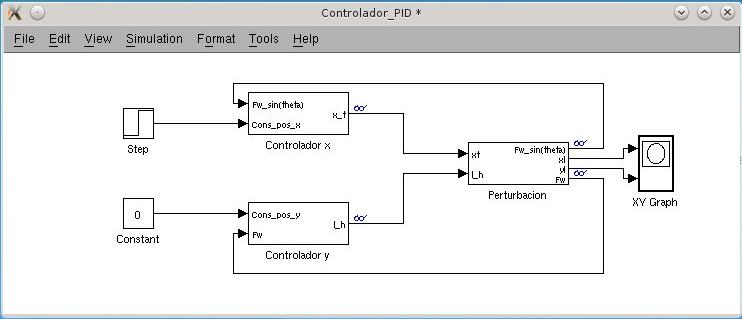
\includegraphics[width=2.5in]{Test_x.jpeg}
  \caption{Modelo Simulink del Controlador de traslación en el eje X}
  \label{fig:testx}
\end{figure}

\begin{figure}[!t]
 \centering
  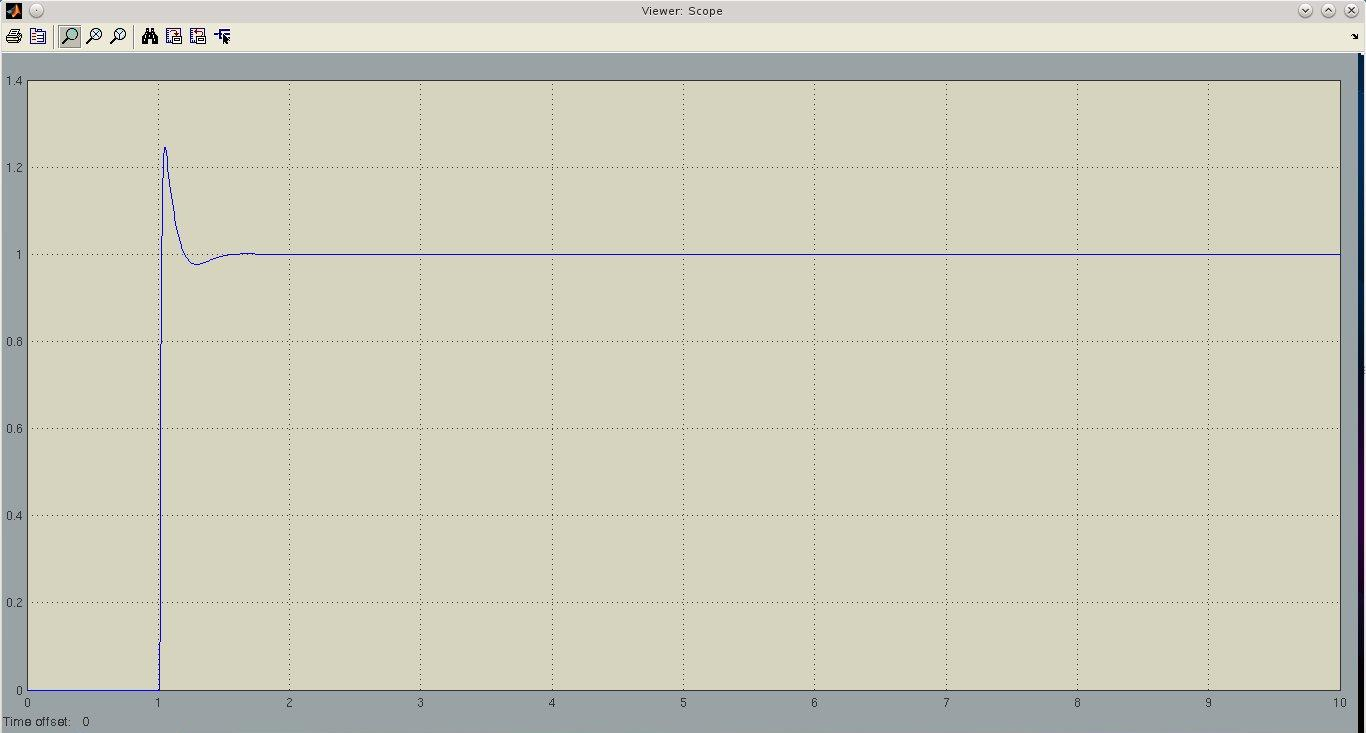
\includegraphics[width=2.5in]{Test_x_posicion.jpeg}
  \caption{Respuesta del sistema a un escalón en el eje X}
  \label{fig:resx}
\end{figure}


\begin{figure}[!t]
 \centering
  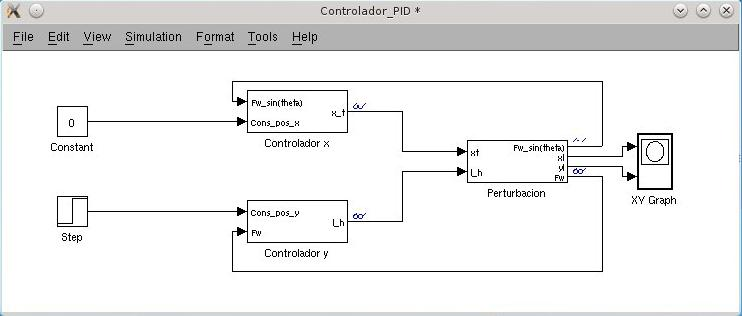
\includegraphics[width=2.5in]{Test_y.jpeg}
  \caption{Modelo Simulink del controlador de izaje en el eje Y}
  \label{fig:testy}
\end{figure}

\begin{figure}[!t]
 \centering
  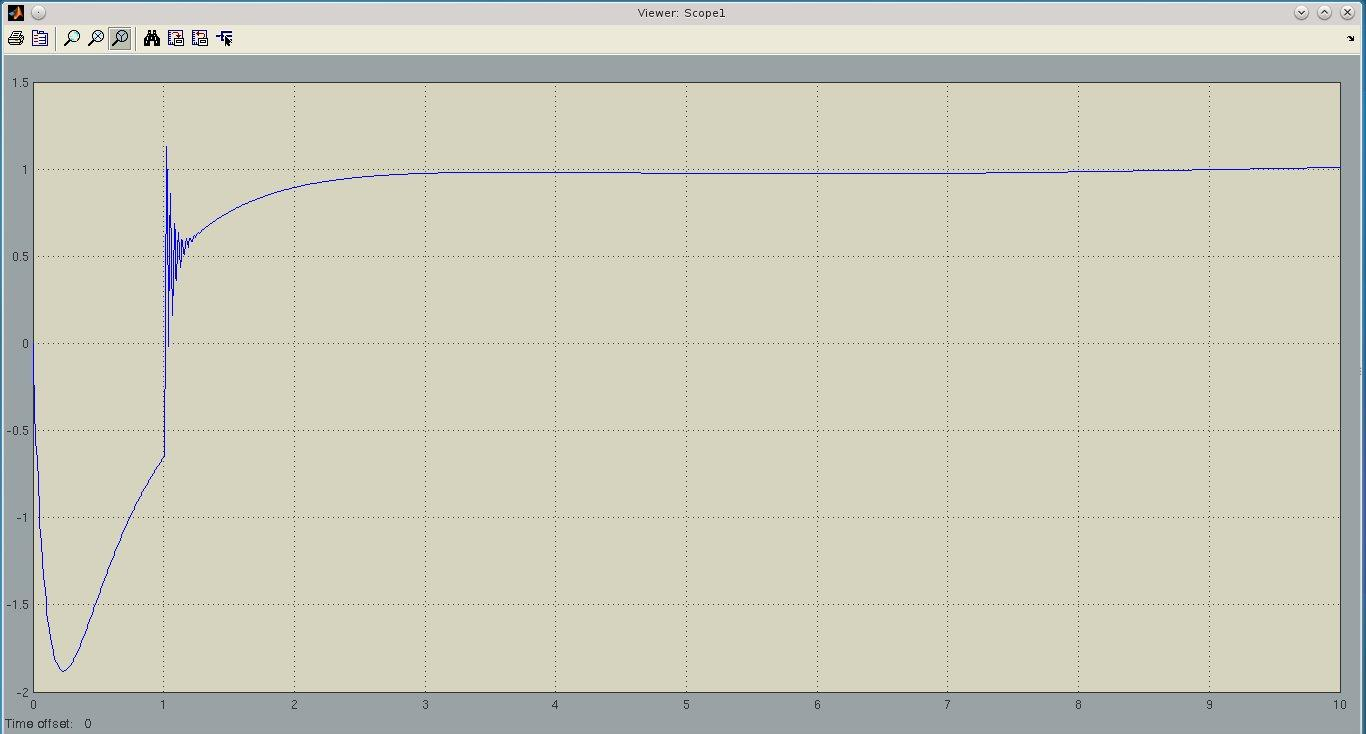
\includegraphics[width=2.5in]{Test_y_posicion.jpeg}
  \caption{Respuesta del sistema a un escalón en el eje Y}
  \label{fig:resy}
\end{figure}

\begin{figure}[!t]
 \centering
  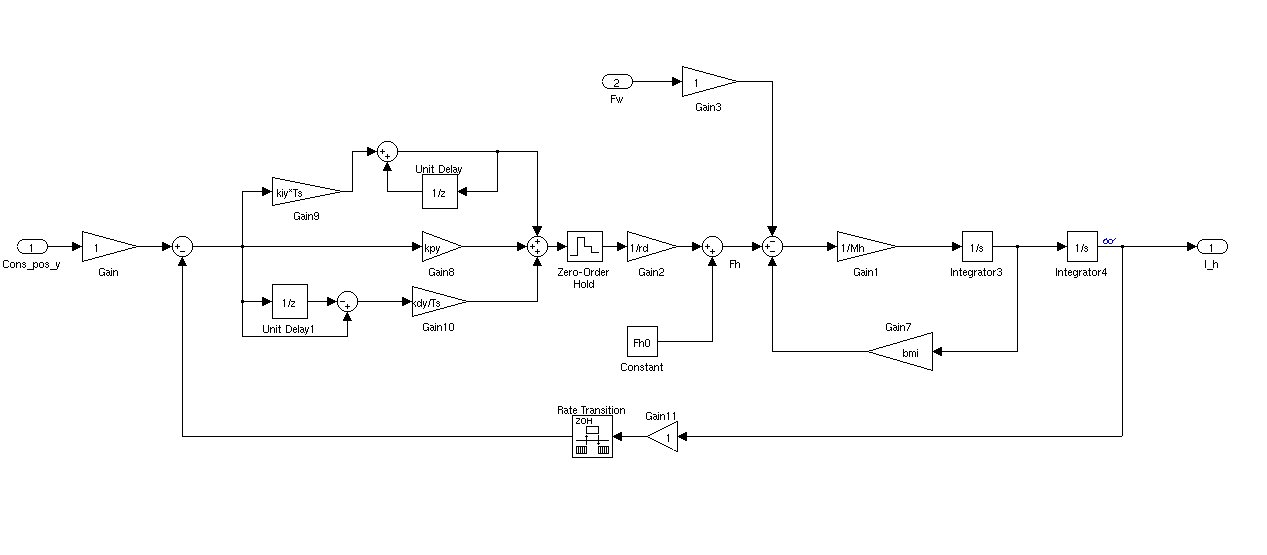
\includegraphics[width=2.5in]{Controlador_precarga.jpeg}
  \caption{Modelo Simulink del controlador de izaje en el eje Y con precarga}
  \label{fig:testyComp}
\end{figure}

\begin{figure}[!t]
 \centering
  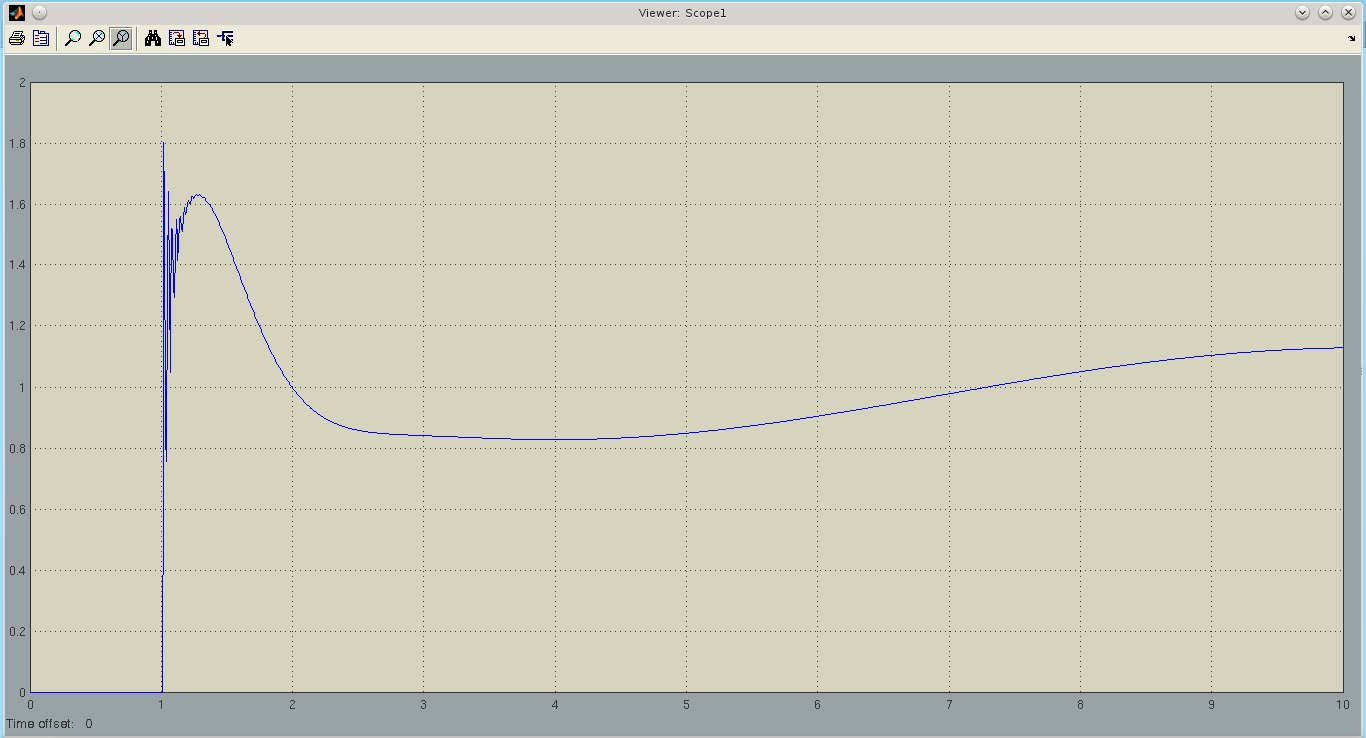
\includegraphics[width=2.5in]{Controlador_prec_res.jpeg}
  \caption{Respuesta del sistema a un escalón en el eje Y con precarga}
  \label{fig:resyComp}
\end{figure}


\subsection{Respuesta con límites de velocidad y aceleración}
Si bien las consignas que la maquina de estados envía al controlador pueden ser representadas
por escalones, se debe cumplir con los límites de velocidad y aceleración del sistema.
Por esta razón, se desea saber como responde el sistema de control ante una consigna en 
escalón que pasa por el sistema de límites de velocidad y aceleración presentados en la 
sección \ref{sec:limites}.


\begin{itemize}
 \item Traslación en el eje $X$. Ver Fig.\ref{fig:consposxxl}.
 
 La máquina de estados enviá una consigna en escalón que el limitador de velocidad y 
 aceleración convierte en una curva. Se observa como la carga sigue a la consigna y el
 movimiento de péndulo de esta.
 \item Izaje en el eje $Y$. Ver Fig.\ref{fig:consposyyl}.
 
  Nuevamente, la consigna en escalón de la maquina de estados al pasar por el limitador de 
  velocidad y aceleración se convierte en una curva. Esta es seguida por el controlador 
  y se puede observar, también, el estiramiento sufrido por el cable.
\end{itemize}

\begin{figure}[!t]
 \centering
  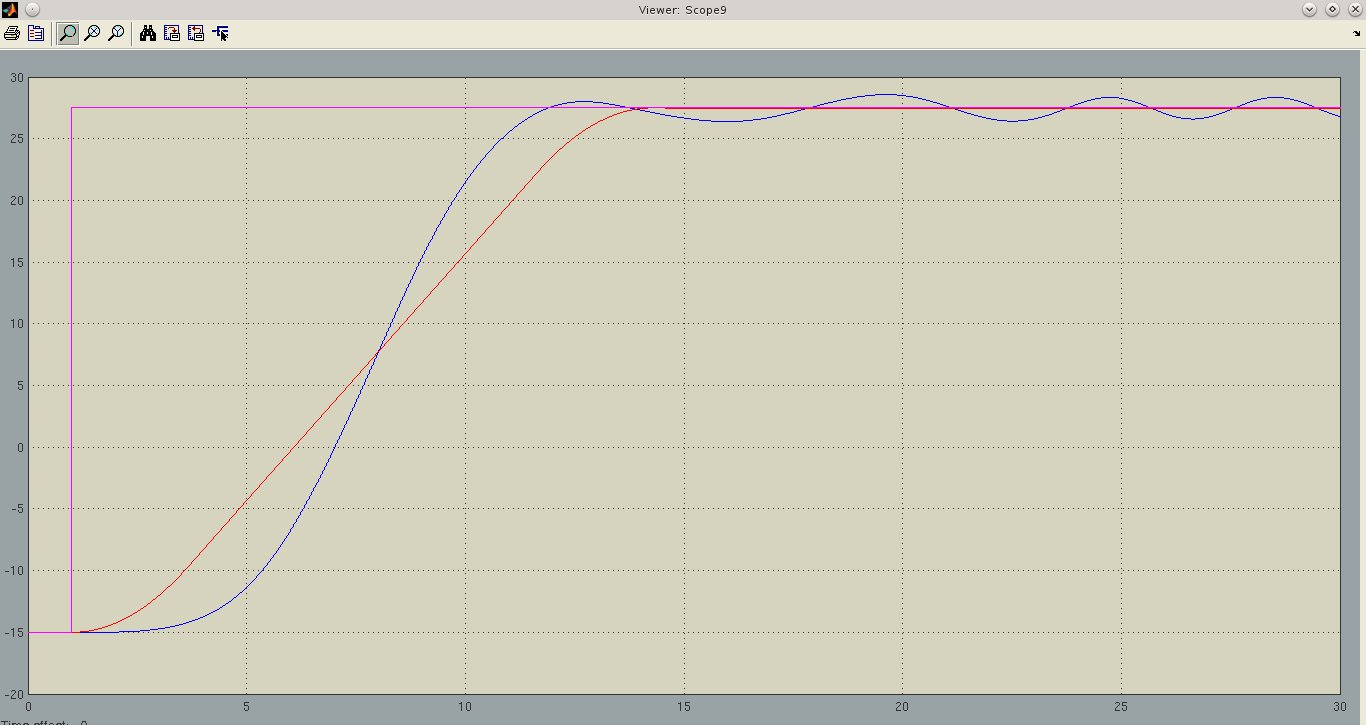
\includegraphics[width=2.5in]{consx_posx_xl.jpeg}
  \caption{Respuesta del sistema y la carga a una perturbación en escalón eje x}
  \label{fig:consposxxl}
\end{figure}

\begin{figure}[!t]
 \centering
  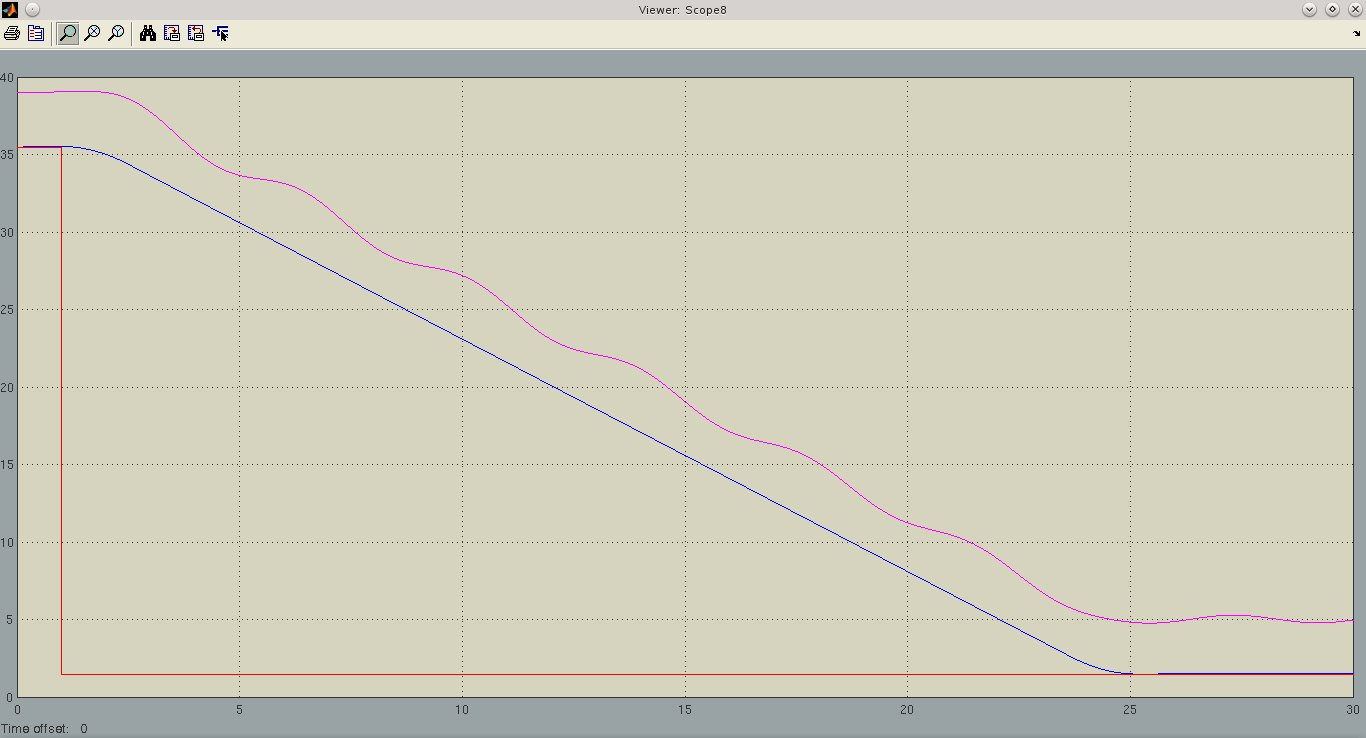
\includegraphics[width=2.5in]{consy_posy_yl.jpeg}
  \caption{Respuesta del sistema y la carga a una perturbación en escalón eje y}
  \label{fig:consposyyl}
\end{figure}


\subsection{Control supervisor de la máquina de estados}
A continuación, se presentan los resultados del trabajo conjunto de la maquina de estados
y los controladores de la traslación e izaje. Es importante marcar que las condiciones 
iniciales en estas demostraciones son las explicadas en la sección \ref{sec:condiniciales}.

\begin{itemize}
 \item Para comenzar la presentación de resultados se muestra en la Fig. \ref{fig:idageneral}
 la respuesta del sistema a un ciclo de ida hacia el barco. Se intenta mostrar con esta imagen
 el sistema de forma global. Se observan las señales enviadas desde la máquina de estados, 
 la respuesta del sistema, así como también el gráfico descripto por la carga en su camino
 hacia el barco en la parte inferior izquierda. También se muestran los switch que representan
 las señales que puede enviarle el operario a la máquina.

\item En la Fig. \ref{fig:consignasyrespuestasy} Se puede observar la consigna en 
escalón enviada desde la máquina de estados, la respuesta de los controladores de 
los motores a la consigna de posición atenuada para estar dentro de los límites de 
velocidad y aceleración como se ve en la figura \ref{fig:atenuaciona} para el izaje
de la carga, mientras que en la Fig. \ref{fig:consignasyrespuestasx} se muestra 
la respuesta en la traslación.

 \item En la Fig. \ref{fig:idavueltageneral} se muestra la respuesta del sistema al 
 movimiento completo. Esto es tomar la carga, realizado de manera manual por el 
 operario, llevarla al barco de manera automática y esperar la señal del operario
 para poder volver al muelle.
 
\end{itemize}

 \begin{figure}[!t]
 \centering
  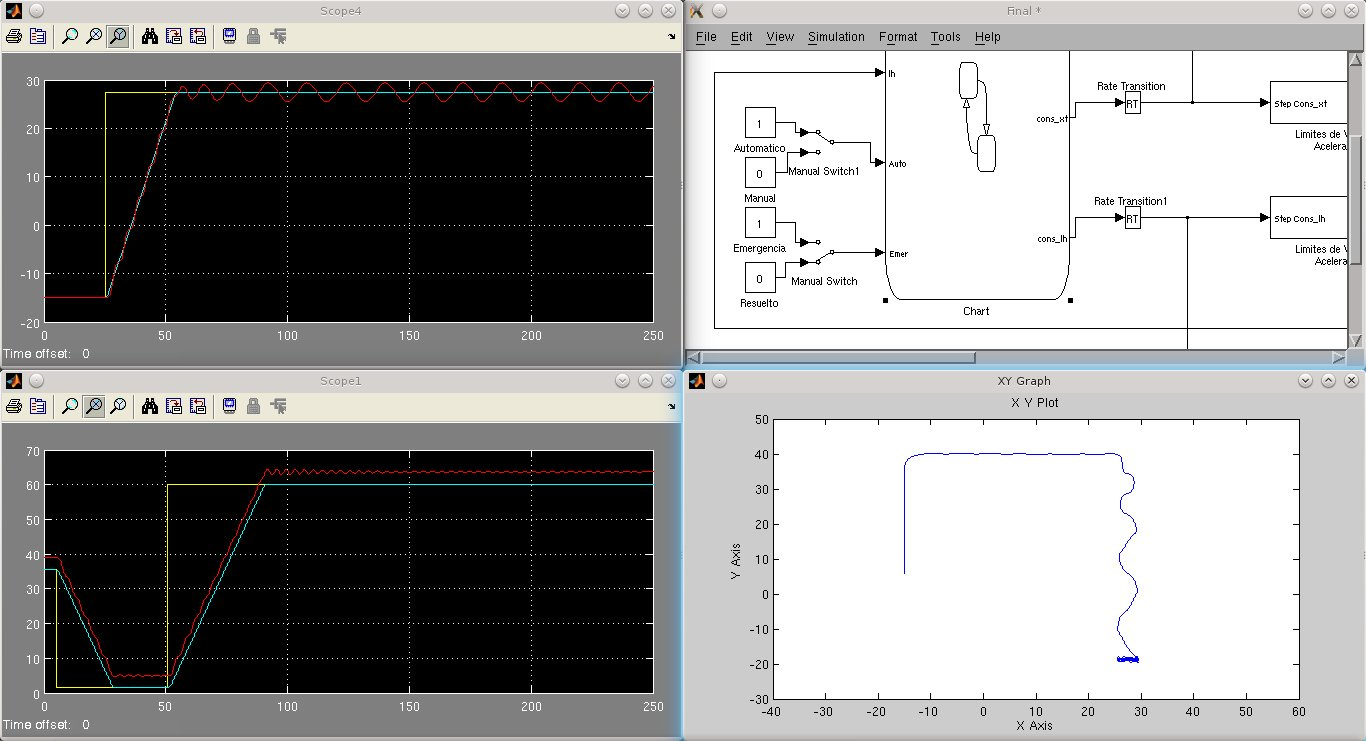
\includegraphics[width=3in]{Ida_general.jpeg}
  \caption{Respuesta del sistema al ciclo de ida hacia el barco}
  \label{fig:idageneral}
\end{figure}

\begin{figure}[!t]
 \centering
  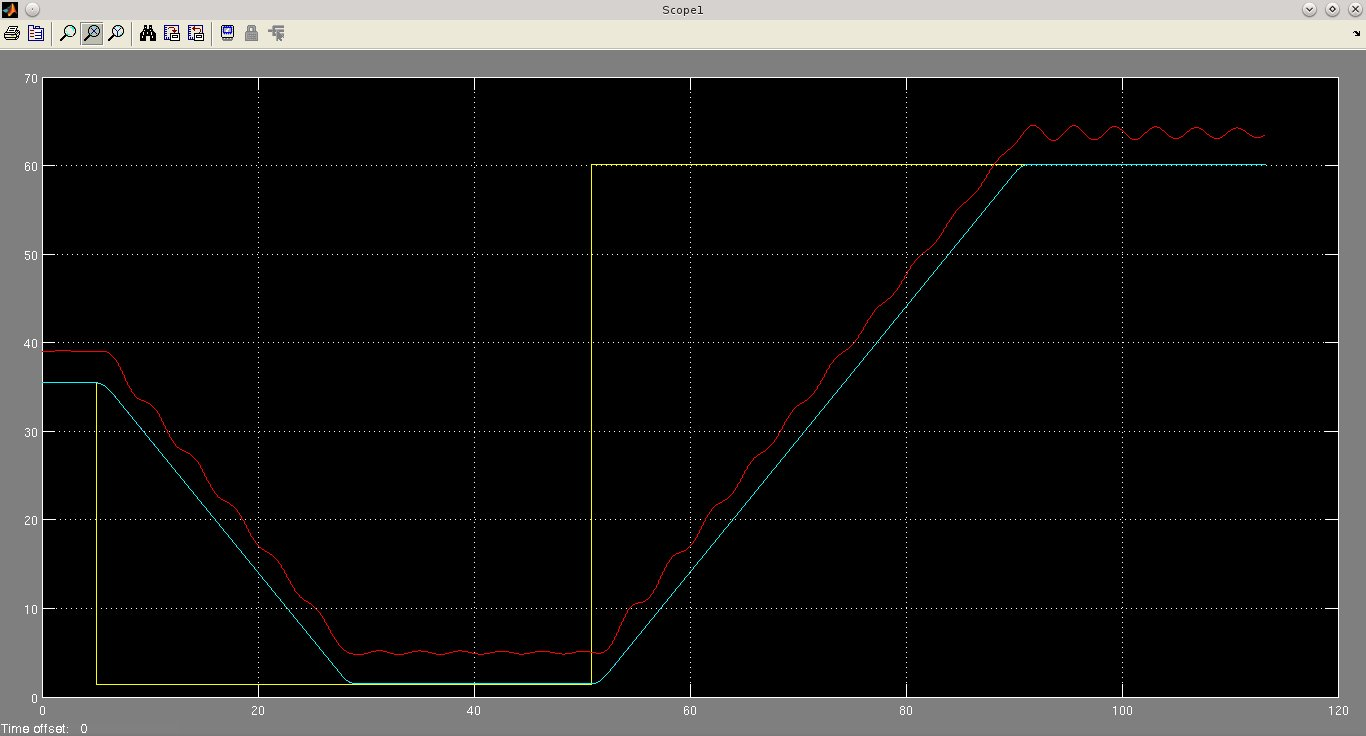
\includegraphics[width=3in]{consignasyrespuestasy.jpeg}
  \caption{Respuesta del sistema al ciclo de ida hacia el barco en el izaje}
  \label{fig:consignasyrespuestasy}
\end{figure}

\begin{figure}[!t]
 \centering
  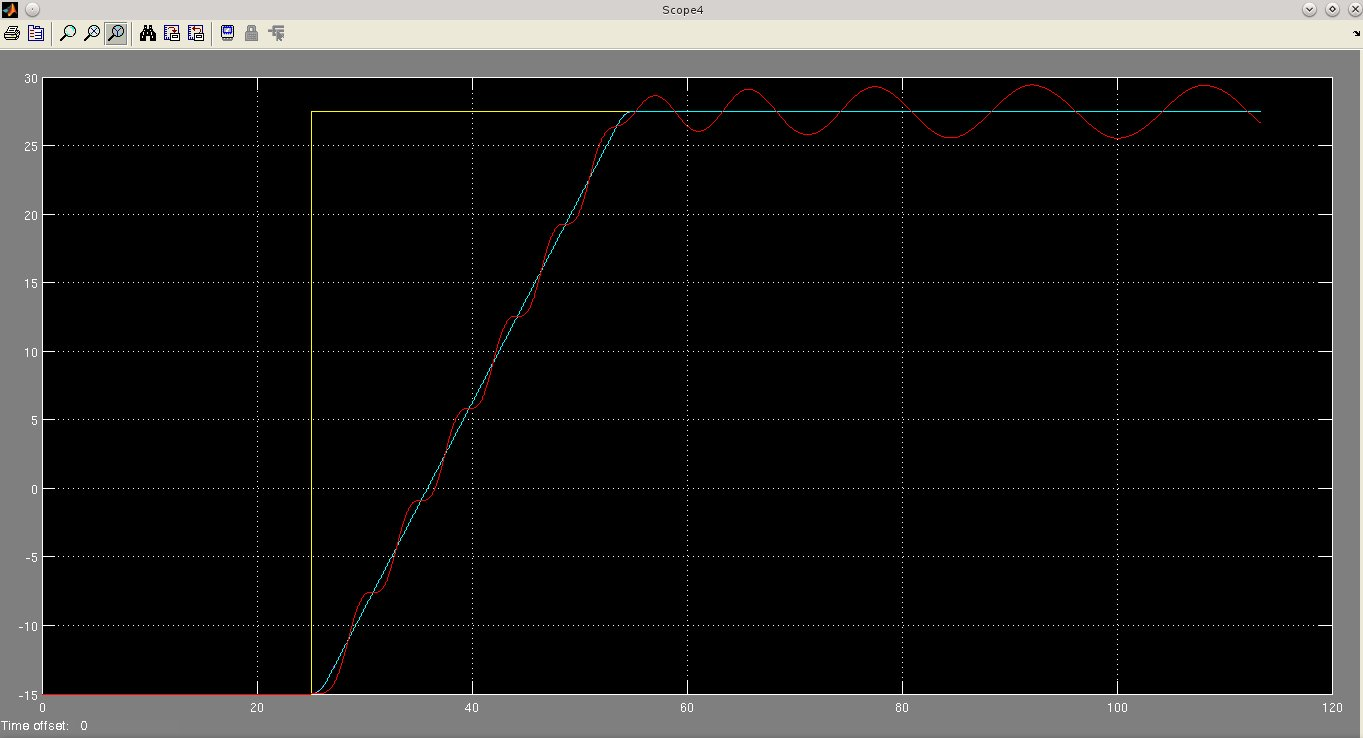
\includegraphics[width=3in]{consignasyrespuestasx.jpeg}
  \caption{Respuesta del sistema al ciclo de ida hacia el barco en traslación}
  \label{fig:consignasyrespuestasx}
\end{figure}

 \begin{figure}[!t]
 \centering
  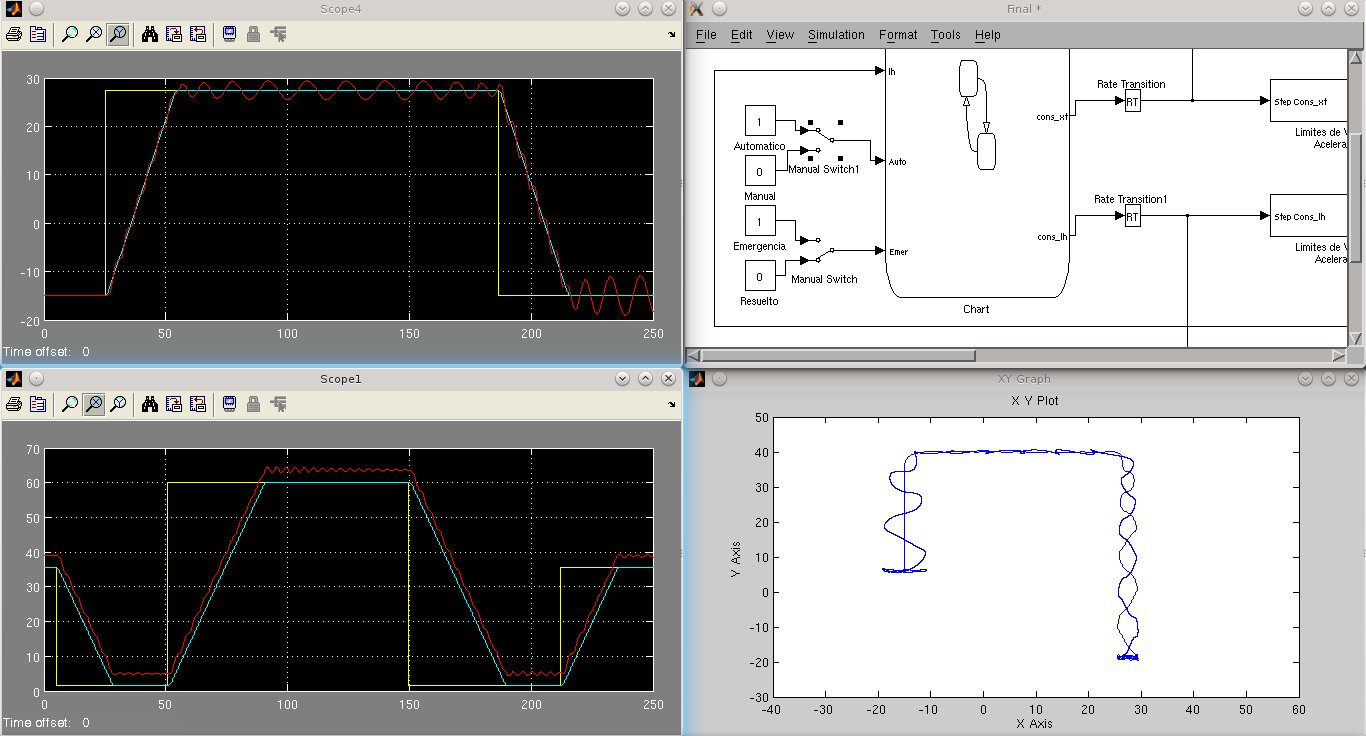
\includegraphics[width=3in]{Ida_vuelta_general.jpeg}
  \caption{Respuesta del sistema a un ciclo de carga completo}
  \label{fig:idavueltageneral}
\end{figure}

\section{Posibles Mejoras}

Hasta ahora tenemos una versión de la máquina de estados que es capaz de esperar 
que el operario tome la carga y automáticamente la lleve al barco y volver desde el
mismo. Se plantean tres mejoras a este modelo que se pueden sumar a nuestro desarrollo
puesto que se han dejado las variables para ello.

\begin{itemize}
 \item inteligencia al estado automático, esto es conocer la posición final de traslación
 teniendo en cuenta dos situaciones:
 \begin{itemize}
  \item Carga secuencial en el eje x, cargar en la columna 1, luego la 2 y así sucesivamente.
  \item Carga completamente la columna 1 y luego completamente la 2 y así sucesivamente.
 \end{itemize}
 
 \item Realizar trayectorias curvas que le permitan al operario que la carga y la descarga 
 se realicen más rápidamente.
 
 \item Detección de carga, discriminando si estamos cargando o descargando, siendo capaces
 de esta manera de avanzar más rápido si no hay carga.
\end{itemize}


\newpage 
\section{Conclusión}
El trabajo tuvo como objetivo realizar un controlador aplicable a los requerimientos
industriales, por ende se tuvieron en cuenta diferentes aspectos de seguridad y 
necesidades que en ese ámbito se requieren.

Es el proyecto integrador de la materia en el que se busco poner en práctica los diferentes
aspectos vistos durante el año.

Hemos destacado dos grande bloques o partes del trabajo:

\begin{itemize}

\item Controlador en tiempo discreto.\\
Es un controlador de más bajo nivel, adaptado como se ha mencionado a las necesidades
digitales.

\item Máquina de estados finitos.\\
Como controlador global, notamos que al programar en este nivel de abstracción, indudablemente
más alto, es mucho más fácil tener en cuenta diferentes situaciones que pueden suceder
en el sistema. 

\end{itemize}

Al trabajar de esta manera pudimos ser capaces de hacer crecer nuestro sistema
de control agregándole estados que solucionaran situaciones 
que en un principio no habíamos tenido en cuenta.

Como resultado del trabajo podemos demostrar las ventajas que presenta realizar máquinas
de estados finitos en problemas en los que pueden existir situaciones concurrentes y
el camino a seguir depende del estado del sistema.

Finalmente, es importante destacar que la seguridad ha sido el factor sobre el que mas 
se ocupo en este trabajo, debido a las graves implicancias que tendría un accidente con este 
tipo de cargas y estructuras.





% if have a single appendix:
%\appendix[Proof of the Zonklar Equations]
% or
%\appendix  % for no appendix heading
% do not use \section anymore after \appendix, only \section*
% is possibly needed

% use appendices with more than one appendix
% then use \section to start each appendix
% you must declare a \section before using any
% \subsection or using \label (\appendices by itself
% starts a section numbered zero.)
%


%\appendices
%\section{Proof of the First Zonklar Equation}
%Appendix one text goes here.

% you can choose not to have a title for an appendix
% if you want by leaving the argument blank
%\section{}
%Appendix two text goes here.


% use section* for acknowledgement
%\section*{Acknowledgment}
%The authors would like to thank...


% Can use something like this to put references on a page
% by themselves when using endfloat and the captionsoff option.
\ifCLASSOPTIONcaptionsoff
  \newpage
\fi



% trigger a \newpage just before the given reference
% number - used to balance the columns on the last page
% adjust value as needed - may need to be readjusted if
% the document is modified later
%\IEEEtriggeratref{8}
% The "triggered" command can be changed if desired:
%\IEEEtriggercmd{\enlargethispage{-5in}}

% references section

% can use a bibliography generated by BibTeX as a .bbl file
% BibTeX documentation can be easily obtained at:
% http://www.ctan.org/tex-archive/biblio/bibtex/contrib/doc/
% The IEEEtran BibTeX style support page is at:
% http://www.michaelshell.org/tex/ieeetran/bibtex/
%\bibliographystyle{IEEEtran}
% argument is your BibTeX string definitions and bibliography database(s)
%\bibliography{IEEEabrv,../bib/paper}
%
% <OR> manually copy in the resultant .bbl file
% set second argument of \begin to the number of references
% (used to reserve space for the reference number labels box)
\begin{thebibliography}{1}

\bibitem{}
Katsuhiko~Ogata, \emph{Modern Control Engineering}, 5th~ed.\relax Editorial:Pearson.
\bibitem{}
Julián Gabriel, \emph{Apuntes y Material de la Cátedra},
\relax Automática y Maquinas Eléctricas, 2013.
\bibitem{}
Julián Gabriel, \emph{Apuntes y Material de la Cátedra},
\relax Autómatas y Control Discreto , 2013.
\bibitem{}
University of Michigan, \emph{Control Tutorials for Matlab \& Simulink},\\
\relax \url{http://ctms.engin.umich.edu/CTMS}.
\end{thebibliography}

% biography section
% 
% If you have an EPS/PDF photo (graphicx package needed) extra braces are
% needed around the contents of the optional argument to biography to prevent 
% the LaTeX parser from getting confused when it sees the complicated
% \includegraphics command within an optional argument. (You could create
% your own custom macro containing the \includegraphics command to make things
% simpler here.)
%\begin{biography}[{\includegraphics[width=1in,height=1.25in,clip,keepaspectratio]{mshell}}]{Michael Shell}
% or if you just want to reserve a space for a photo:

%\begin{IEEEbiography}{Michael Shell}
%Biography text here.
%\end{IEEEbiography}

% if you will not have a photo at all:
%\begin{IEEEbiographynophoto}{John Doe}
%Biography text here.
%\end{IEEEbiographynophoto}

% insert where needed to balance the two columns on the last page with
% biographies
%\newpage

%\begin{IEEEbiographynophoto}{Jane Doe}
%Biography text here.
%\end{IEEEbiographynophoto}

% You can push biographies down or up by placing
% a \vfill before or after them. The appropriate
% use of \vfill depends on what kind of text is
% on the last page and whether or not the columns
% are being equalized.

%\vfill

% Can be used to pull up biographies so that the bottom of the last one
% is flush with the other column.
%\enlargethispage{-5in}



% that's all folks
\end{document}


